\documentclass[output=paper]{langscibook}
\ChapterDOI{10.5281/zenodo.15006613}
\author{Margje Post\orcid{}\affiliation{University of Bergen}}
\title[Regional prosodic variation in the speech of young urban Russians]{Regional prosodic variation in the speech of young urban Russians: Quantitative vowel reduction in Moscow and Perm}

\abstract{Most young urban Russians speak with little or no local characteristics in their speech, but small regional differences in segmental and prosodic properties are likely to be present. In order to find out whether regional prosodic differences persist in modern urban speech, we compared durational vowel reduction in the speech of adolescents from the capital Moscow and from Perm (Ural). In contemporary Central Standard Russian, non-high vowels in first pretonic position are much less reduced than other unstressed vowels. This reduction in two degrees is strong in Central Russia, but the difference between the degrees appears to be smaller in other parts of the country. Our study shows a large and stable difference in reduction patterns between the two cities, for both male and female speakers, even though it is based on read speech, which tends to be closer to standard language, with less local traits, than other speaking styles.}
\IfFileExists{../localcommands.tex}{
  \addbibresource{../localbibliography.bib}
  \usepackage{tabularx,multicol}
%\usepackage{multirow}
\usepackage{subcaption}
\usepackage{url}
\urlstyle{same}

\usepackage{datetime}
\usepackage{enumitem}
\usepackage{langsci-optional}
\usepackage{langsci-lgr}
\usepackage{langsci-branding}

\usepackage{longtable}
\usepackage{xltabular}
\usepackage[linguistics, edges]{forest}
\usepackage{pgfplots}
\pgfplotsset{compat=1.18}
\usetikzlibrary{patterns, tikzmark}
\usepackage{pgfplotstable}
\usepgfplotslibrary{colorbrewer}
\usepackage{listings}
\lstset{basicstyle=\ttfamily,keywordstyle=\normalfont,language=,breaklines=true}

\usepackage{siunitx}
\sisetup{group-digits=none, detect-all=true}

\usepackage{langsci-gb4e}

  \makeatletter
\let\thetitle\@title
\let\theauthor\@author
\makeatother

% Use this Chinese font shipped with TeX Live instead of Source Han, because
% it is more portable/leightweight. Install the "fandol" package from CTAN to
% automatically get this font.
\newfontfamily{\ChineseFandolSong}{FandolSong-Regular.otf}

  %% hyphenation points for line breaks
%% Normally, automatic hyphenation in LaTeX is very good
%% If a word is mis-hyphenated, add it to this file
%%
%% add information to TeX file before \begin{document} with:
%% %% hyphenation points for line breaks
%% Normally, automatic hyphenation in LaTeX is very good
%% If a word is mis-hyphenated, add it to this file
%%
%% add information to TeX file before \begin{document} with:
%% %% hyphenation points for line breaks
%% Normally, automatic hyphenation in LaTeX is very good
%% If a word is mis-hyphenated, add it to this file
%%
%% add information to TeX file before \begin{document} with:
%% \include{localhyphenation}
\hyphenation{
    a-na-ly-sis
    ap-proach-es
    ar-che-o-log-i-cal
    Ar-khan-gelsk
    be-schrei-ben
    Buch-holtz
    Che-lya-binsk
    con-so-nant
    dia-lect
    dia-lect-ology
    Di-a-lekt-for-schung
    Dia-lekt-for-schung
    East-pha-lian
    För-der-ung
    Ge-mein-schaft-lich-keits-ent-wür-fe
    his-tor-i-cal
    Hok-kai-do
    ja-pa-nese
    Ja-pa-nese
    Ka-go-shi-ma
    Ka-li-nin-grad
    Knja-zev
    Ma-kro-be-reich
    Ma-lay-sia
    mor-pho-log-i-cal
    Mos-cow
    Nef-te-yu-gansk
    non-mobile
    nu-cle-ar
    ös-ter-rei-chi-sche
    par-a-digm
    per-zep-ti-ons-lin-gu-is-ti-sche
    plu-ri-zen-tri-schen
    quick-ly
    Reich
    Sax-on
    Schrö-der
    sear-ching
    ste-reo-type
    strength-en-ing
    strong-est
    Stutt-gart
    su-pra-seg-men-tal
    teach-er
    to-po-gra-phy
    To-ron-to
    tra-di-tion-al
    ul-ti-mate-ly
    Um-gangs-spra-che
    Volks-kun-de
    vor-zu-stel-len
    wheth-er
    Wie-sing-er
    with-in
    Wort-at-las
}

\hyphenation{
    a-na-ly-sis
    ap-proach-es
    ar-che-o-log-i-cal
    Ar-khan-gelsk
    be-schrei-ben
    Buch-holtz
    Che-lya-binsk
    con-so-nant
    dia-lect
    dia-lect-ology
    Di-a-lekt-for-schung
    Dia-lekt-for-schung
    East-pha-lian
    För-der-ung
    Ge-mein-schaft-lich-keits-ent-wür-fe
    his-tor-i-cal
    Hok-kai-do
    ja-pa-nese
    Ja-pa-nese
    Ka-go-shi-ma
    Ka-li-nin-grad
    Knja-zev
    Ma-kro-be-reich
    Ma-lay-sia
    mor-pho-log-i-cal
    Mos-cow
    Nef-te-yu-gansk
    non-mobile
    nu-cle-ar
    ös-ter-rei-chi-sche
    par-a-digm
    per-zep-ti-ons-lin-gu-is-ti-sche
    plu-ri-zen-tri-schen
    quick-ly
    Reich
    Sax-on
    Schrö-der
    sear-ching
    ste-reo-type
    strength-en-ing
    strong-est
    Stutt-gart
    su-pra-seg-men-tal
    teach-er
    to-po-gra-phy
    To-ron-to
    tra-di-tion-al
    ul-ti-mate-ly
    Um-gangs-spra-che
    Volks-kun-de
    vor-zu-stel-len
    wheth-er
    Wie-sing-er
    with-in
    Wort-at-las
}

\hyphenation{
    a-na-ly-sis
    ap-proach-es
    ar-che-o-log-i-cal
    Ar-khan-gelsk
    be-schrei-ben
    Buch-holtz
    Che-lya-binsk
    con-so-nant
    dia-lect
    dia-lect-ology
    Di-a-lekt-for-schung
    Dia-lekt-for-schung
    East-pha-lian
    För-der-ung
    Ge-mein-schaft-lich-keits-ent-wür-fe
    his-tor-i-cal
    Hok-kai-do
    ja-pa-nese
    Ja-pa-nese
    Ka-go-shi-ma
    Ka-li-nin-grad
    Knja-zev
    Ma-kro-be-reich
    Ma-lay-sia
    mor-pho-log-i-cal
    Mos-cow
    Nef-te-yu-gansk
    non-mobile
    nu-cle-ar
    ös-ter-rei-chi-sche
    par-a-digm
    per-zep-ti-ons-lin-gu-is-ti-sche
    plu-ri-zen-tri-schen
    quick-ly
    Reich
    Sax-on
    Schrö-der
    sear-ching
    ste-reo-type
    strength-en-ing
    strong-est
    Stutt-gart
    su-pra-seg-men-tal
    teach-er
    to-po-gra-phy
    To-ron-to
    tra-di-tion-al
    ul-ti-mate-ly
    Um-gangs-spra-che
    Volks-kun-de
    vor-zu-stel-len
    wheth-er
    Wie-sing-er
    with-in
    Wort-at-las
}

  \togglepaper[1]%%chapternumber
}{}

\begin{document}
\graphicspath{{figures/post}}
\maketitle
\label{chap:post}
% ATTENTION: Diacritics on the following phonetic characters might have been lost during conversion: {'ə'}




\section{Introduction}
\label{sec:post:1}
\subsection{Regional variation in Russian}
\label{sec:post:1.1}
Russian is a language with little geographically based variation, compared to other languages, and the Russian-speaking community has a strong standard language ideology. The dialectal differences have never been large, and, with the strong centralization tendencies in Russia and expectations to speak proper, standard Russian, most young urban Russians speak with little or no local features in their speech. It is often assumed that educated Russians have a standard pronunciation without local characteristics. However, most researchers acknowledge the existence of locally coloured varieties of Standard Russian (\citealt{Panov1967, Krysin2007, Andrews2006, Krause2010, GrammatčikovaPožarickaja2013}).\footnote{Cyrillic script is latinised following \citegen{ComrieCorbett1993} transliteration system, apart from toponyms, where the usual English forms are used (Moscow, Perm, Chelyabinsk).} The local features in regionally coloured standard speech are mainly restricted to lexical items and minor differences in pronunciation.\footnote{In \citegen{Auer2005} standard-dialect constellations in European languages, Russian is classified among the languages with so-called diaglossia, which have a continuum between rural dialects and the standard language (cf. \citealt{Krause2010}), but Russian is at best a poor example of diaglossia. Little is known about the intermediate space between base dialects and the standard. The traditional rural dialects are under strong pressure, and, although the term regiolect is in use for Russian (see discussion in \citealt{Krause2010}), stable intermediate regional varieties appear to be absent or rare.}



When so little variation is heard in public space, it is no surprise that today’s youth in Russia, according to a recent folk linguistic study, has restricted knowledge of regional variation in Russian \citep{Vardøy2021}. \citet[72]{GrammatčikovaPožarickaja2013} claim nevertheless that Russians can often, after hearing the first word, distinguish speakers from different cities. One can expect, along with Grammatčikova and her colleagues, that much of the ability to recognise a speaker’s regional provenance can be accounted for by regional differences in prosody (\citealt{GrammatčikovaPožarickaja2013, Post2017}). \citet{ErofeevaEtAl2000} get the impression that prosodic characteristics are the most important cue to the local colouring of speech from the city of Perm, despite its numerous local characteristics on the segmental level \citep{Erofeeva2005}. However, little is known about the phonetics of regional varieties of Standard Russian, let alone about their prosody. As remarked by \citet{Kalenčuk2021}, sociolinguistic studies of regional variants of standard language pronunciation have hardly been conducted. Linguists usually describe only the Moscow and Petersburg norm, and codify only the Moscow norm, based on the idea formulated by Vasilij Černyšev back in 1915 that ``educated people in all parts of Russia speak Moscow Russian'' \citep[11]{Kalenčuk2021}. Following \citet[522]{Iosad2012}, I will call this Central Russian norm \textit{contemporary Central Standard Russian} (CSR).


\subsection{Vowel reduction and prosodic word structure in Russian}
\label{sec:post:1.2}
\subsubsection{Central Standard Russian: Strong nucleus and reduction in two degrees}
\label{sec:post:1.2.1}
One of the areas with known regional variation is in the expression of unstressed vowels. Russian has mobile, distinctive stress -- word stress can occur on any syllable of the word; cf. \textit{{}zámok} `castle' vs. \textit{zamók} `lock'; \textit{{}kólokol} \textsc{nom.sg} `bell' vs. \textit{kolokolá} \textsc{nom.pl} `bells'. Vowel length is not phonologically contrastive. Instead, it plays an important role in the expression and perception of stress \citep[219]{Bondarko1998}. Unstressed vowels are subject to reduction. Most notably, unstressed \mbox{/o/} merges with \mbox{/a/}, so the words \textit{travá} [trɐˈva] ‘grass, herb’ and \textit{drová} [drɐˈva] ‘firewood’ are pronounced with the same vowels. In addition, Central Standard Russian (CSR) has a typologically unusual word prosodic pattern with a heavy nucleus and weak periphery: the first pretonic syllable -- i.e., the syllable immediately preceding the stressed syllable -- is uncommonly prominent, especially when it contains an open vowel; cf. the [ɐ] in \textit{travá} and \textit{drová}. This syllable forms a salient contrast, together with the stressed syllable, with unstressed syllables in other, weak positions, which are heavily reduced, both in quality and quantity (\citealt{Zlatoustova1981, Kodzasov1999}). In addition, the first pretonic syllable is often singled out by a local high tone \citep{Kasatkina2005}. One could argue that word stress is realised over two syllables, as \citet[175]{Dubina2012} claims about Belarusian. This uncommon prominence of the first pretonic vowel leads to vowel reduction in two degrees, called \textit{moderate} and \textit{radical} reduction by \citet{Crosswhite2000}, with moderate, degree 1 reduction occurring in the first pretonic syllable and strong, degree 2 reduction elsewhere.\footnote{Moderate, degree 1 reduction is also found in other positions that allow long vowel durations, notably, in onsetless syllables and, optionally, in phrase-final open syllables (\citealt{Barnes2006}, \citealt[534]{Iosad2012}). \citet{Kuznecov1997} discerns an additional, third degree of quantitative reduction for posttonic vowels, based on the statistics of his phonetic study.} In CSR, the word \textit{molokó} `milk' is typically pronounced [mәlɐˈko], with a short \textit{schwa} in the second pretonic syllable (= radical reduction), and a long, open vowel in first pretonic position (= moderate reduction). Following \citet{Potebnja1866}, we can describe the distribution of syllable prominence in the word in CSR by the formula \mbox{112ˈ311}, where 1 means radical reduction, 2 means moderate reduction and ˈ3 stands for no reduction in the stressed syllable. Empirical studies of CSR have confirmed that Potebnja’s \mbox{112ˈ311} formula corresponds to a three-way distinction in duration (e.g., \citealt{BondarkoEtAl1966, Zlatoustova1981, Kuznecov1997, Barnes2006, Knjazev2006}). The durational differences between the syllables relative to stress are highest for non-high vowels (\citealt{Zlatoustova1981, BondarkoEtAl1966}), i.e., for unstressed /a, o/ after non-palatalised consonants. Only for these vowels a qualitative distinction between the two positions into two different allophones is discerned. This two-degree qualitative reduction of unstressed /a, o/ into [ɐ] and [ә] is incorporated into the prescriptive pronunciation standard \citep{Avanesov1984}.\footnote{Most older literature uses the symbol [ʌ] for the first degree reduction of /a, o/ after non-palatalised consonants; cf. \citet{Iosad2012} for a discussion.} It is also an integral part of Russian L2 course books.\footnote{This is not restricted to books at the university level. An example of a Russian L2 course book for secondary schools where two-degree reduction is taught, is \citet{HertzEtAl2005}.} The two-degree reduction in duration, however, is not mentioned.



Due to this typologically uncommon reduction pattern, vowel reduction in Russian is a well-known and much studied area in phonetics and phonology.\footnote{Examples of empirical phonetic research on vowel reduction in CSR are \citet{Zlatoustova1981}, \citet{BondarkoEtAl1966}, \citet{Kuznecov1997}, \citet{PadgettTabain2005}, \citet{Barnes2006}, \citet{KocharovEtAl2015}. Examples of phonological accounts are \citet{Crosswhite2000}, \citet{Iosad2012}, \citet{Mołczanow2015}.} Most literature is based on, and accounts for, Central Standard Russian speech. Although two-degree reduction in duration is claimed to be a common feature of East Slavic \citep{Dubina2012}, the difference between degree 1 and degree 2 varies. The next sections will discuss the durational reduction patterns in other varieties of Russian.


\subsubsection{Traditional Russian rural dialects}
\label{sec:post:1.2.2}
As to traditional rural dialects, the first pretonic prominence -- and the related two-degree reduction -- varies from very prominent in some Central Russian dialect groups (in which the rhythmic structure can be described as 113ˈ311 according to Potebnja’s formulae, e.g., group V in \figref{fig:post:1}), to (almost) absent in parts of the Russian North (111ˈ211; group VIII in \figref{fig:post:1}). \citet{GrammatčikovaPožarickaja2013} state that some dialects do not have a prosodic nucleus of the first pretonic and tonic syllable at all, but \citet{Vysotskij1973} claims that all traditional Russian dialects have it to some degree (\citeyear[34,36]{Vysotskij1973}).\footnote{The fact that Vysotskij found a durational difference between the second and first pretonic vowels in all dialects does not necessarily entail that they all have two-degree reduction, at least not at a phonological level. Besides, some of the recorded speakers might have accommodated their speech to the interview situation and have spoken with more two-degree reduction than they would have done when speaking with locals. \citet{Paufošima1978} suspects some of her dialect speakers of trying to copy the word rhythm of perceived Standard Russian, with some being more successful at this than others.} \citet{Vysotskij1973} measured the rhythmic word structure in a large number of Russian rural dialects by examining consonant and vowel durations. He distinguishes 15 varieties of Russian, both rural dialects and varieties of Russian spoken in Moscow, which all have a different word rhythm pattern. The durations in a selection of these groups are given in \figref{fig:post:1}.

\begin{figure}[h]
    \pgfplotsset{
    	/pgfplots/bar cycle list/.style={/pgfplots/cycle list={
    			{black,fill=black!90!white,mark=none},
    			{black!80,fill=black!60!white,mark=none},
    			{black!60,fill=black!10!white,mark=none},
    		},
    	},
    }
\begin{subfigure}{\textwidth}
    \pgfplotstableread{data/post-figure1.csv}\PostFigureOneData
    \begin{tikzpicture}
	\small
	\begin{axis}
		[
            axis lines*=left,
			bar width=2.75ex,
			font=\small,
			height=5cm,
			legend cell align=left,
			nodes near coords,
			width=\textwidth,
			xtick=data,
			xticklabels from table={\PostFigureOneData}{Data},
			x tick label style={text width=1.25cm, align=center, font=\sloppy\small},
			y tick label style={font=\small},
            ybar=3pt,
			ylabel=ms,
			ylabel near ticks,
			ymin=0,
		]
		\foreach \i in {2nd pretonic,1st pretonic,tonic (stressed)}
		  {
		  	\addplot table [x expr=\coordindex, x=Data, y=\i] {\PostFigureOneData};
		    \edef\temp{\noexpand\addlegendentry{\i}}
		    \temp
 		  }
	\end{axis}
    \end{tikzpicture}
    \caption{Mean absolute vowel durations (from \protect\citealt{Vysotskij1973})}
\end{subfigure}\medskip\\
% % % 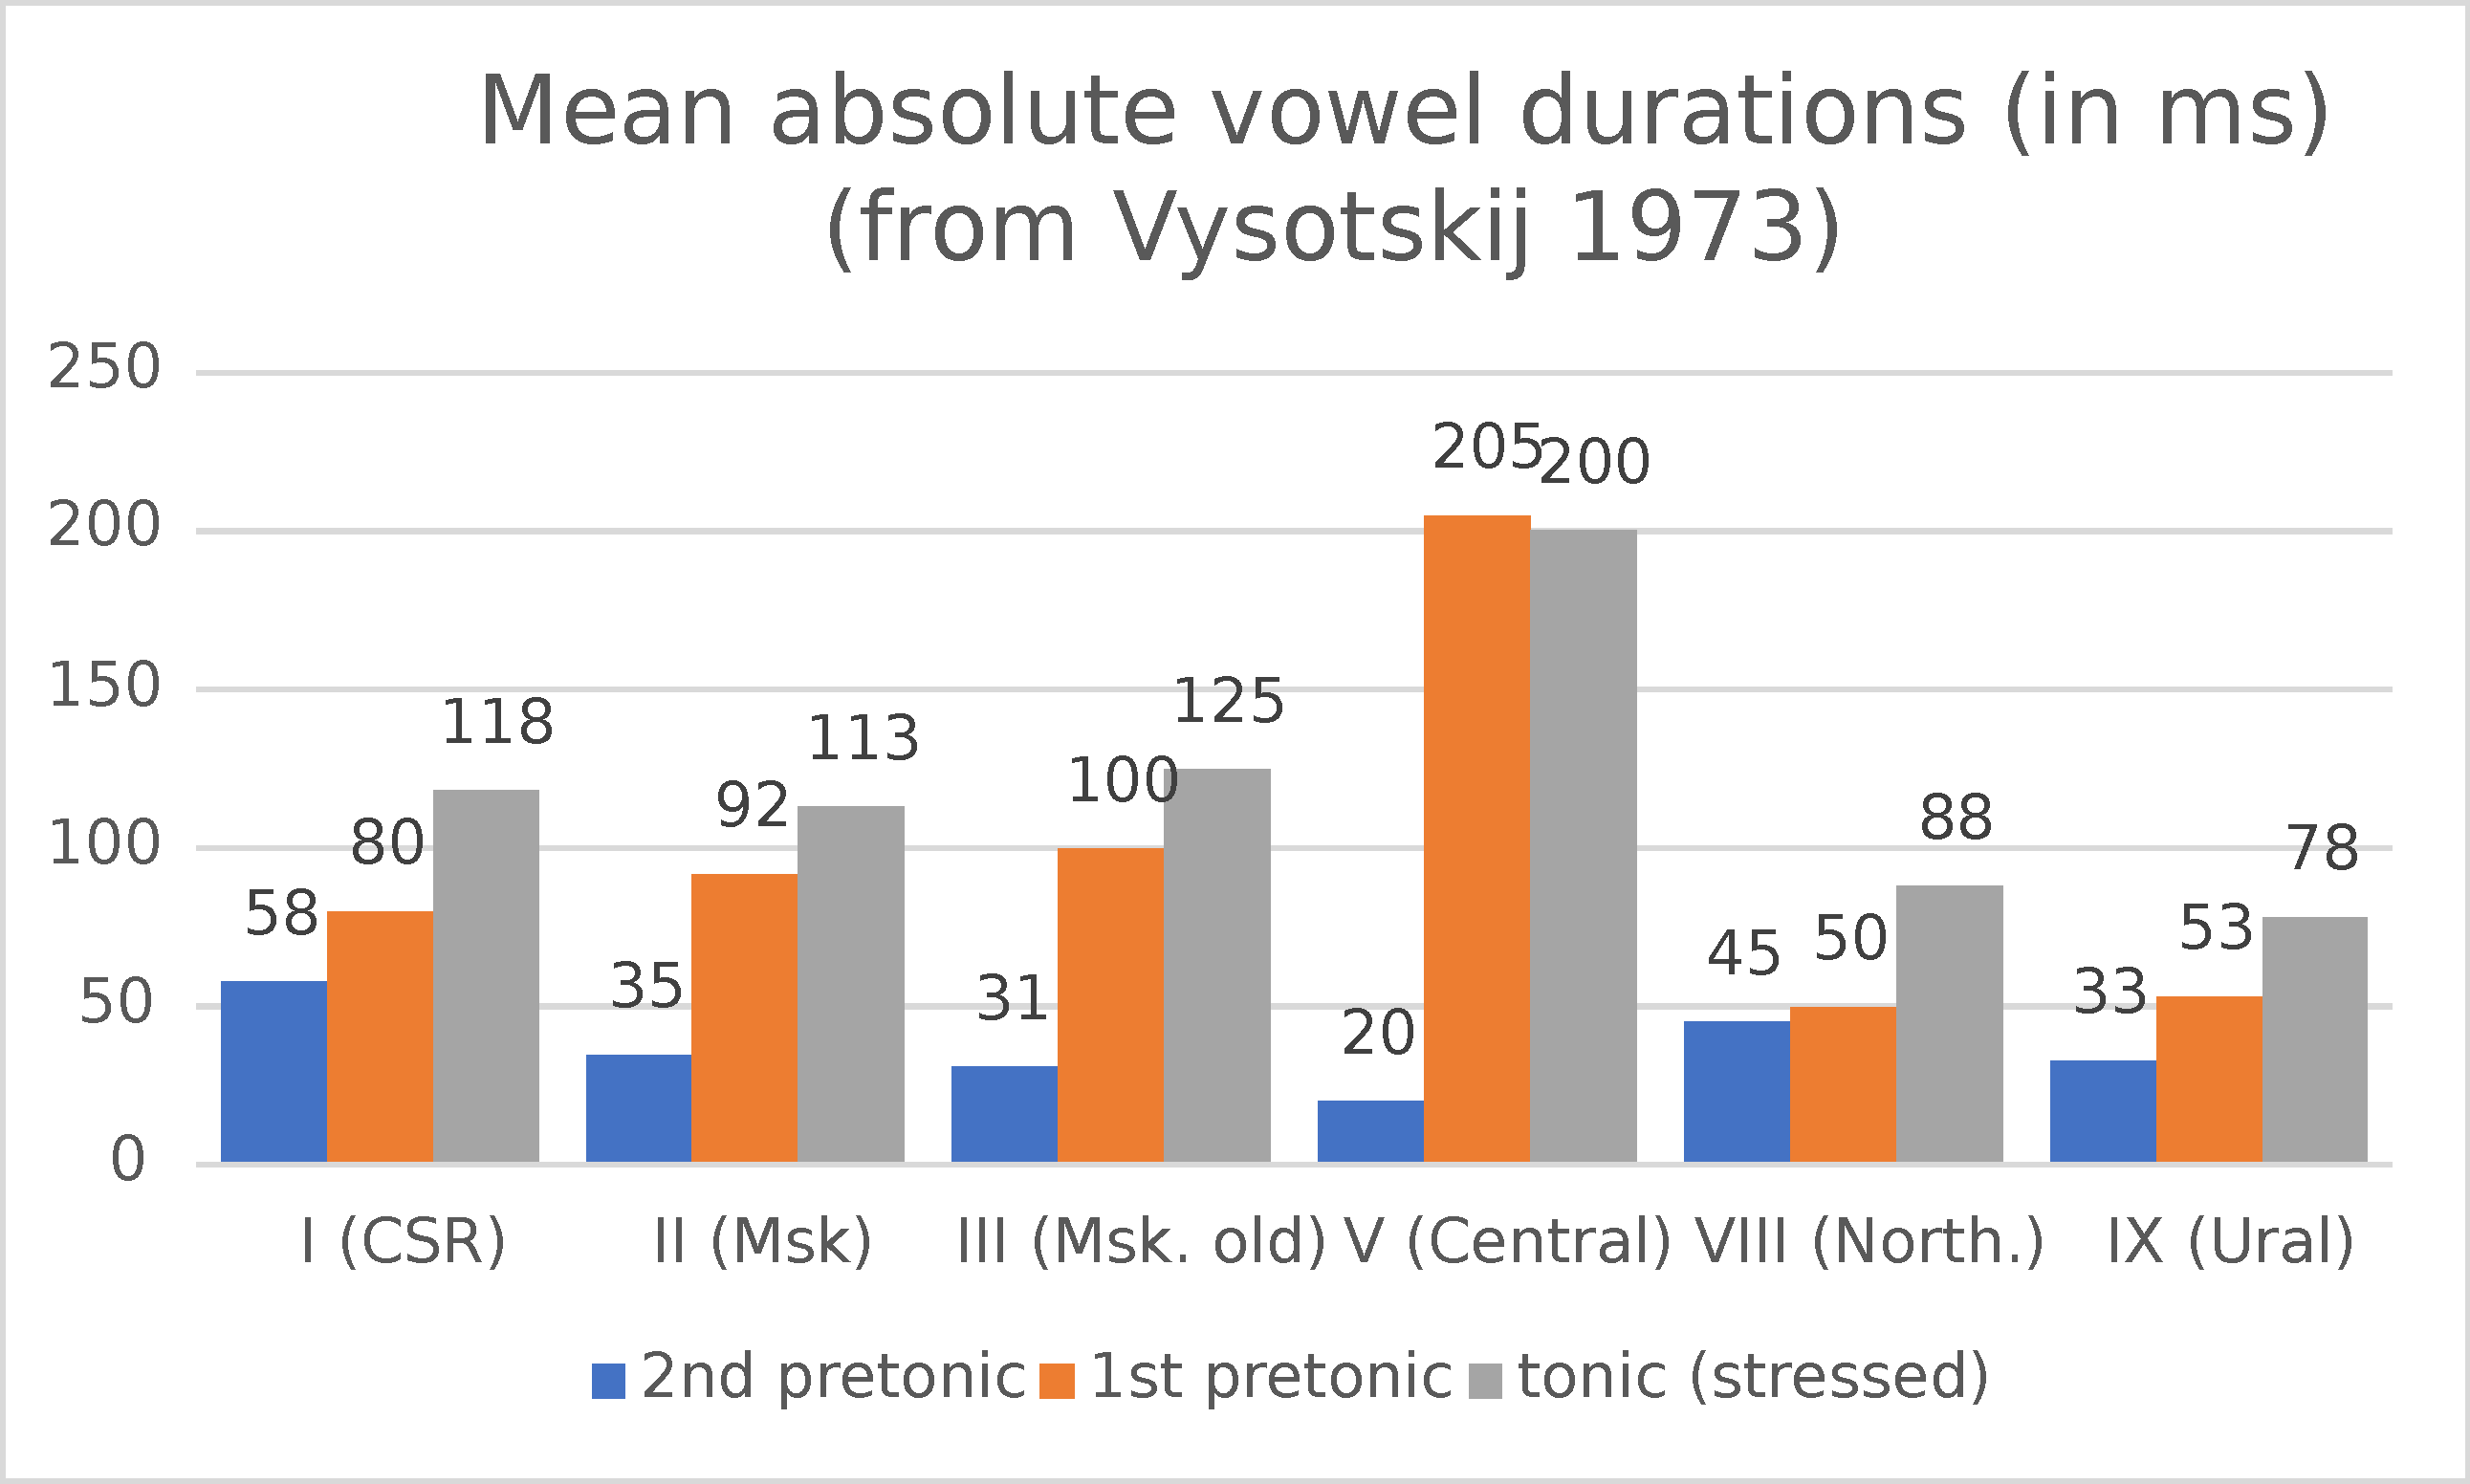
\includegraphics[width=\textwidth]{PostFig1A vowel dur vysotskij absol.pdf}
\begin{subfigure}{\textwidth}
\pgfplotstableread{data/post-figure1b.csv}\PostFigureOneBData
    \begin{tikzpicture}
	\small
	\begin{axis}
		[
            axis lines*=left,
			bar width=6ex,
			font=\small,
			height=5cm,
			width=\textwidth,
			xtick=data,
			xticklabels from table={\PostFigureOneBData}{Data},
			x tick label style={text width=1.25cm, align=center, font=\sloppy\small},
			y tick label style={font=\small},
            ybar stacked, %=3pt,
			ylabel=\%,
			ylabel near ticks,
			ymin=0,
			ymax=100,
			ymajorgrids=true
		]
		\foreach \i in {2nd pretonic,1st pretonic,tonic (stressed)}
		  {
		  	\addplot table [x expr=\coordindex, x=Data, y=\i] {\PostFigureOneBData};
% 		    \edef\temp{\noexpand\addlegendentry{\i}}
% 		    \temp
 		  }
     \end{axis}
     \end{tikzpicture}
% % % 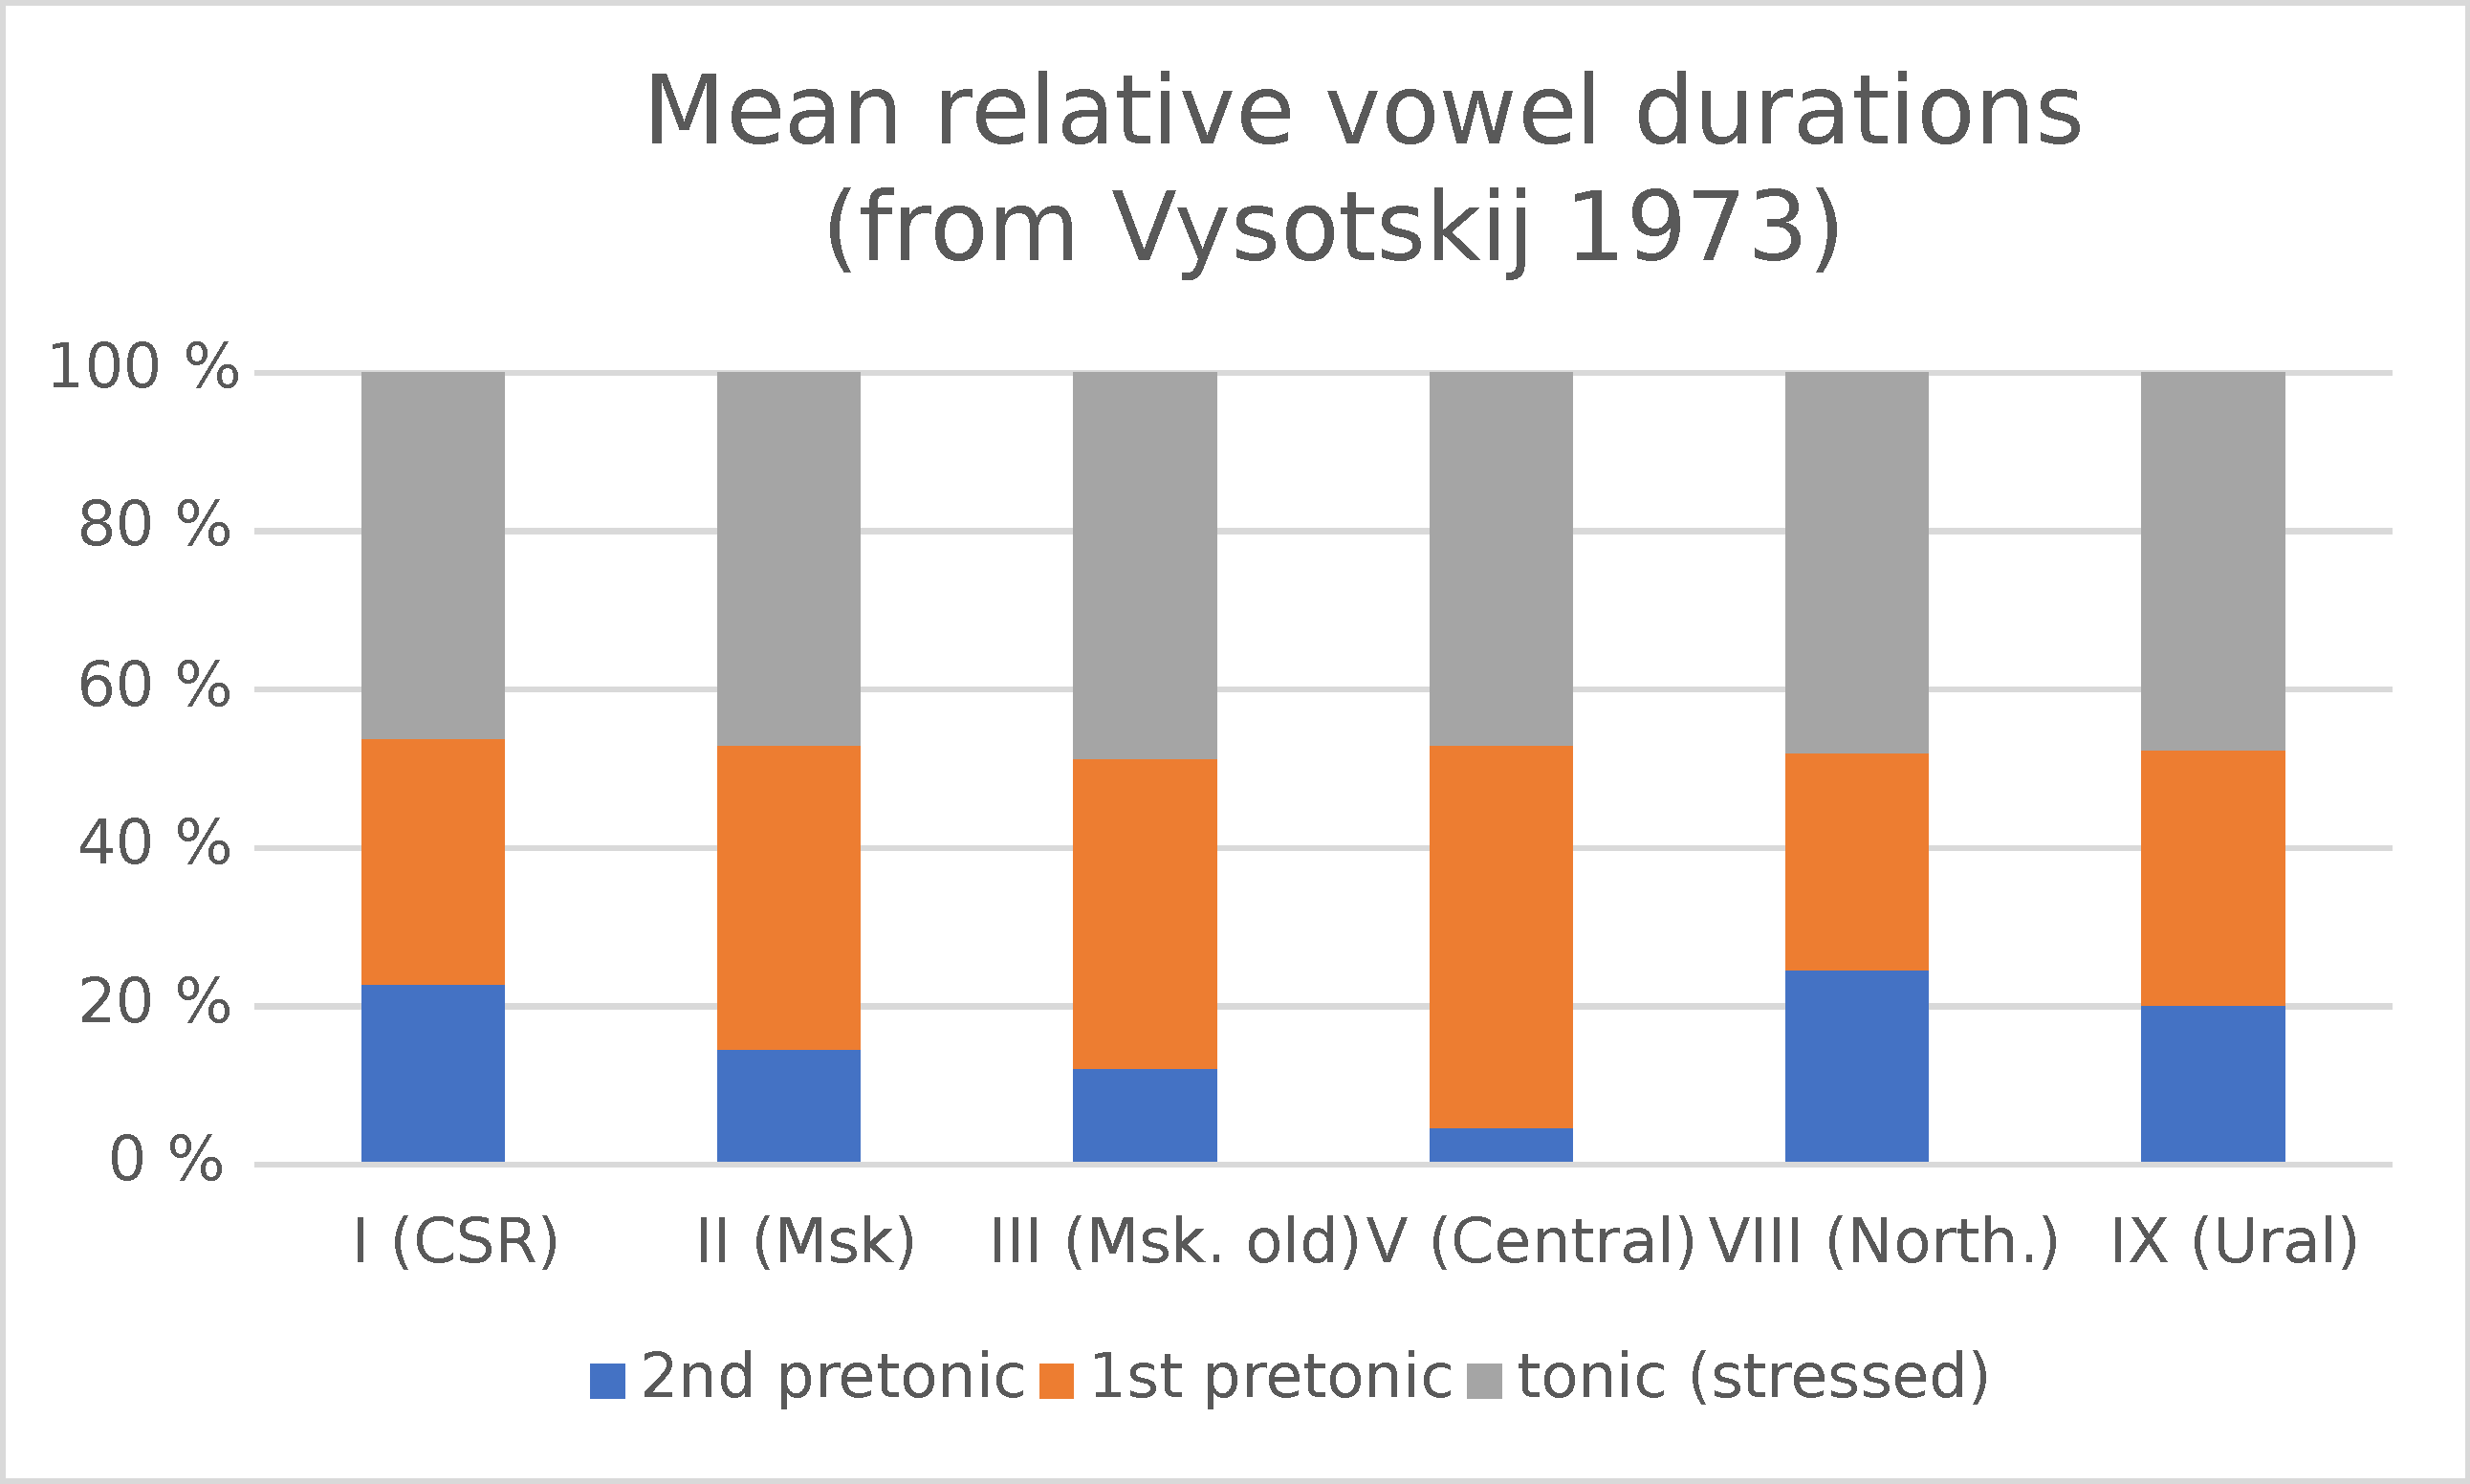
\includegraphics[width=\textwidth]{PostFig1B vowel dur vysotskij relat.pdf}
\caption{Mean vowel durations relative to the total vowel duration in the word (from \protect\citealt{Vysotskij1973})}
\end{subfigure}
\caption{\label{fig:post:1}Mean vowel durations in second pretonic, first pretonic and tonic (stressed) position, in Standard Russian pronunciation (CSR, group I), in Moscow vernacular speech (group II), in the old Moscow norm (III) and in three dialect groups (V, VIII and IX), from \citet[38]{Vysotskij1973}, partly also in \citet[131]{Bethin2006}. The vowels are /o, a/ after non-palatalised plosives and fricatives in words with the structure CV-CV-ˈCVC, in utterance-final and utterance-medial position. Vysotskij measured 100–150 word tokens per speaker (\citeyear[33]{Vysotskij1973}), but it is not clear if more than one speaker per group was analysed.}
\end{figure}

The most extreme groups are group V and group VIII. In group V, found in the Vladimir-Volga basin in Central Russia (discussed by \citealt{Bethin2006}: 113), the durations of the second and first pretonic vowels are extremely different. Group VIII, on the other hand, situated in the North of European Russia, shows hardly any difference between the pretonic vowels. The remaining 13 groups in Vysotskij’s study have intermediate values, including Standard Russian, which is Vysotskij’s type I (\figref{fig:post:1}, first group). Type II represents the Moscow vernacular, with a larger two-degree difference than in CSR (group I). Group III shows the old Moscow norm, with an even larger difference, closer to the rural Central Russian dialects. Finally, group XI is included in \figref{fig:post:1} because it represents the Ural region, where we recorded part of our own data (see \sectref{sec:post:1.3} below).

In a large area in Southwestern Russia, and in a neighbouring region across the border in Belarus and Ukraine, the vowel reduction pattern is complicated by vowel dissimilation. In these dialects, the quality and duration of the first pretonic vowel, and in some cases its tone, depend on the quality of the stressed syllable, for the two neighbouring vowels must be different in both quality and quantity.\footnote{In dialects with vowel dissimilation, a stressed low vowel [a] is never preceded by a low vowel, but by a mid vowel \textit{schwa}, whereas high vowels are preceded by a low vowel. The low vowels are substantially longer than the high vowels, leading to a length trade-off between first pretonic and tonic vowel (see \citealt{Čekmonas2001, Almuxamedova1985, Kasatkina2005, Bethin2006, Savinov2013, Djačenko2015} for studies of dialects with dissimilative vowel systems that take into account their duration). \citet{Iosad2012} suggests that all vowel dissimilation is first and foremost a dissimilation in length. Speakers from Moscow have no qualitative dissimilation, but clear quantitative dissimilation: a length trade-off between first pretonic and tonic vowel, for the first pretonic low vowels have by far the longest duration when preceding short, stressed high vowels (\citealt{Kasatkina2005, Iosad2012}).}


\subsubsection{Modern urban Russian}
\label{sec:post:1.2.3}
Most speakers of Russian today do not speak a traditional rural dialect, however. A handful of studies have addressed ongoing phonological changes in rural areas of Russia, among them \citet{Paufošima1978} on a Northern dialect and \citet{Kochetov2006} on rural speech from the Perm area. As to modern urban Russian, there might still be differences in relative vowel durations between speakers from Moscow and St. Petersburg, although most differences between Moscow and St. Petersburg speech that have been reported in older literature have disappeared, as \citet{Verbickaja1977} found out in a phonetic study of the speech of 150 speakers from St. Petersburg (Leningrad) and 50 speakers from Moscow -- at least between educated speakers in formal settings. In Verbickaja’s study, the two-degree reduction is still somewhat stronger in Moscow than in Saint Petersburg standard speech, due to its relatively shorter vowels in second pretonic and posttonic position (\citealt{Verbickaja1977}, see also \citealt{Nikolaeva1977, Kuznecov1997}). 



\citet{PadgettTabain2005} found substantial interspeaker variation in the expression of two-degree reduction among speakers of Standard Russian, which might be due to differences in geographical provenance. They recorded speakers of Standard Russian living in Australia with various geographical provenance, tacitly assuming that people who are assessed to speak standard Russian, have the same pronunciation. Their participants from Moscow, Saint Petersburg and Kiev had larger, and clearly categorical, differences in duration than their other participants, who were born in China or had a mixed geographical background (\citealt[42]{PadgettTabain2005}, Fig. 4). However, a speaker of Russian does not have to grow up in Central Russia to express strong two-degree reduction: The difference between the vowels was very large for Barnes’ participant from Ufa, the capital of Bashkortostan \citep{Barnes2006}.



Two preliminary studies have measured unstressed vowel durations in large cities other than Moscow and Saint Petersburg (\citealt{GrammatčikovaPožarickaja2013, Erofeeva2005}). Both studies suggest that the geographical opposition between centre and periphery is retained in modern urban Russian -- with strong two-degree reduction in Central Russia, but a lesser difference between the two degrees in non-central areas of the country.



\citet{GrammatčikovaPožarickaja2013} measured vowel durations in trisyllabic words with a Ca\textsubscript{$-2$}C a\textsubscript{$-1$}Cá\textsubscript{0}C structure in a text, read by students from different parts of Russia, and compared them to the pronunciation by a middle-aged Moscow speaker of Standard Russian. In the speech of the Moscow speaker, the first pretonic vowel was not uncommonly long in absolute terms, but it had the longest duration relative to the second pretonic and tonic vowels (\figref{fig:post:2}, page~\pageref{fig:post:2}). The 5 students from other cities had smaller relative differences. One should take into account that these data are preliminary, based on a small number of vowel tokens by only 6 speakers.


\begin{figure}
    \pgfplotsset{
    	/pgfplots/bar cycle list/.style={/pgfplots/cycle list={
    			{black,fill=black!90!white,mark=none},
    			{black!80,fill=black!60!white,mark=none},
    			{black!60,fill=black!10!white,mark=none},
    		},
    	},
    }
\begin{subfigure}{\textwidth}
    \pgfplotstableread{data/post-figure2a.csv}\PostFigureTwoAData
    \begin{tikzpicture}
	\small
	\begin{axis}
		[
            axis lines*=left,
			bar width=2.5ex,
			font=\small,
			height=6cm,
			enlarge y limits={value=0.2,upper},
			legend cell align=left,
			nodes near coords,
			width=\textwidth,
			xtick=data,
			xticklabels from table={\PostFigureTwoAData}{Data},
			x tick label style={text width=1.25cm, align=center, font=\sloppy\small},
			y tick label style={font=\small},
            ybar=3pt,
			ylabel=ms,
			ylabel near ticks,
			ymin=0,
		]
		\foreach \i in {2nd pretonic,1st pretonic,tonic (stressed)}
		  {
		  	\addplot table [x expr=\coordindex, x=Data, y=\i] {\PostFigureTwoAData};
		    \edef\temp{\noexpand\addlegendentry{\i}}
		    \temp
 		  }
	\end{axis}
    \end{tikzpicture}
    \caption{Mean vowel durations in CVCVˈCV(CV) words (from \protect\citealt{GrammatčikovaPožarickaja2013}; Perm (sp) from \protect\citealt{Erofeeva2005})}
\end{subfigure}\medskip\\
\begin{subfigure}{\textwidth}
\pgfplotstableread{data/post-figure2b.csv}\PostFigureTwoBData
    \begin{tikzpicture}
	\small
	\begin{axis}
		[
            axis lines*=left,
			bar width=6ex,
			font=\small,
			height=5cm,
			width=\textwidth,
			xtick=data,
			xticklabels from table={\PostFigureTwoBData}{Data},
			x tick label style={text width=1.25cm, align=center, font=\sloppy\small},
			y tick label style={font=\small},
            ybar stacked, %=3pt,
			ylabel=\%,
			ylabel near ticks,
			ymin=0,
			ymax=100,
			ymajorgrids=true
		]
		\foreach \i in {2nd pretonic,1st pretonic,tonic (stressed)}
		  {
		  	\addplot table [x expr=\coordindex, x=Data, y=\i] {\PostFigureTwoBData};
% 		    \edef\temp{\noexpand\addlegendentry{\i}}
% 		    \temp
 		  }
     \end{axis}
     \end{tikzpicture}
\caption{Vowel durations relative to the total vowel duration in CVCVˈCV(CV) words
(from \protect\citealt{GrammatčikovaPožarickaja2013}; Perm (sp) from \protect\citealt{Erofeeva2005})}
\end{subfigure}
% % % 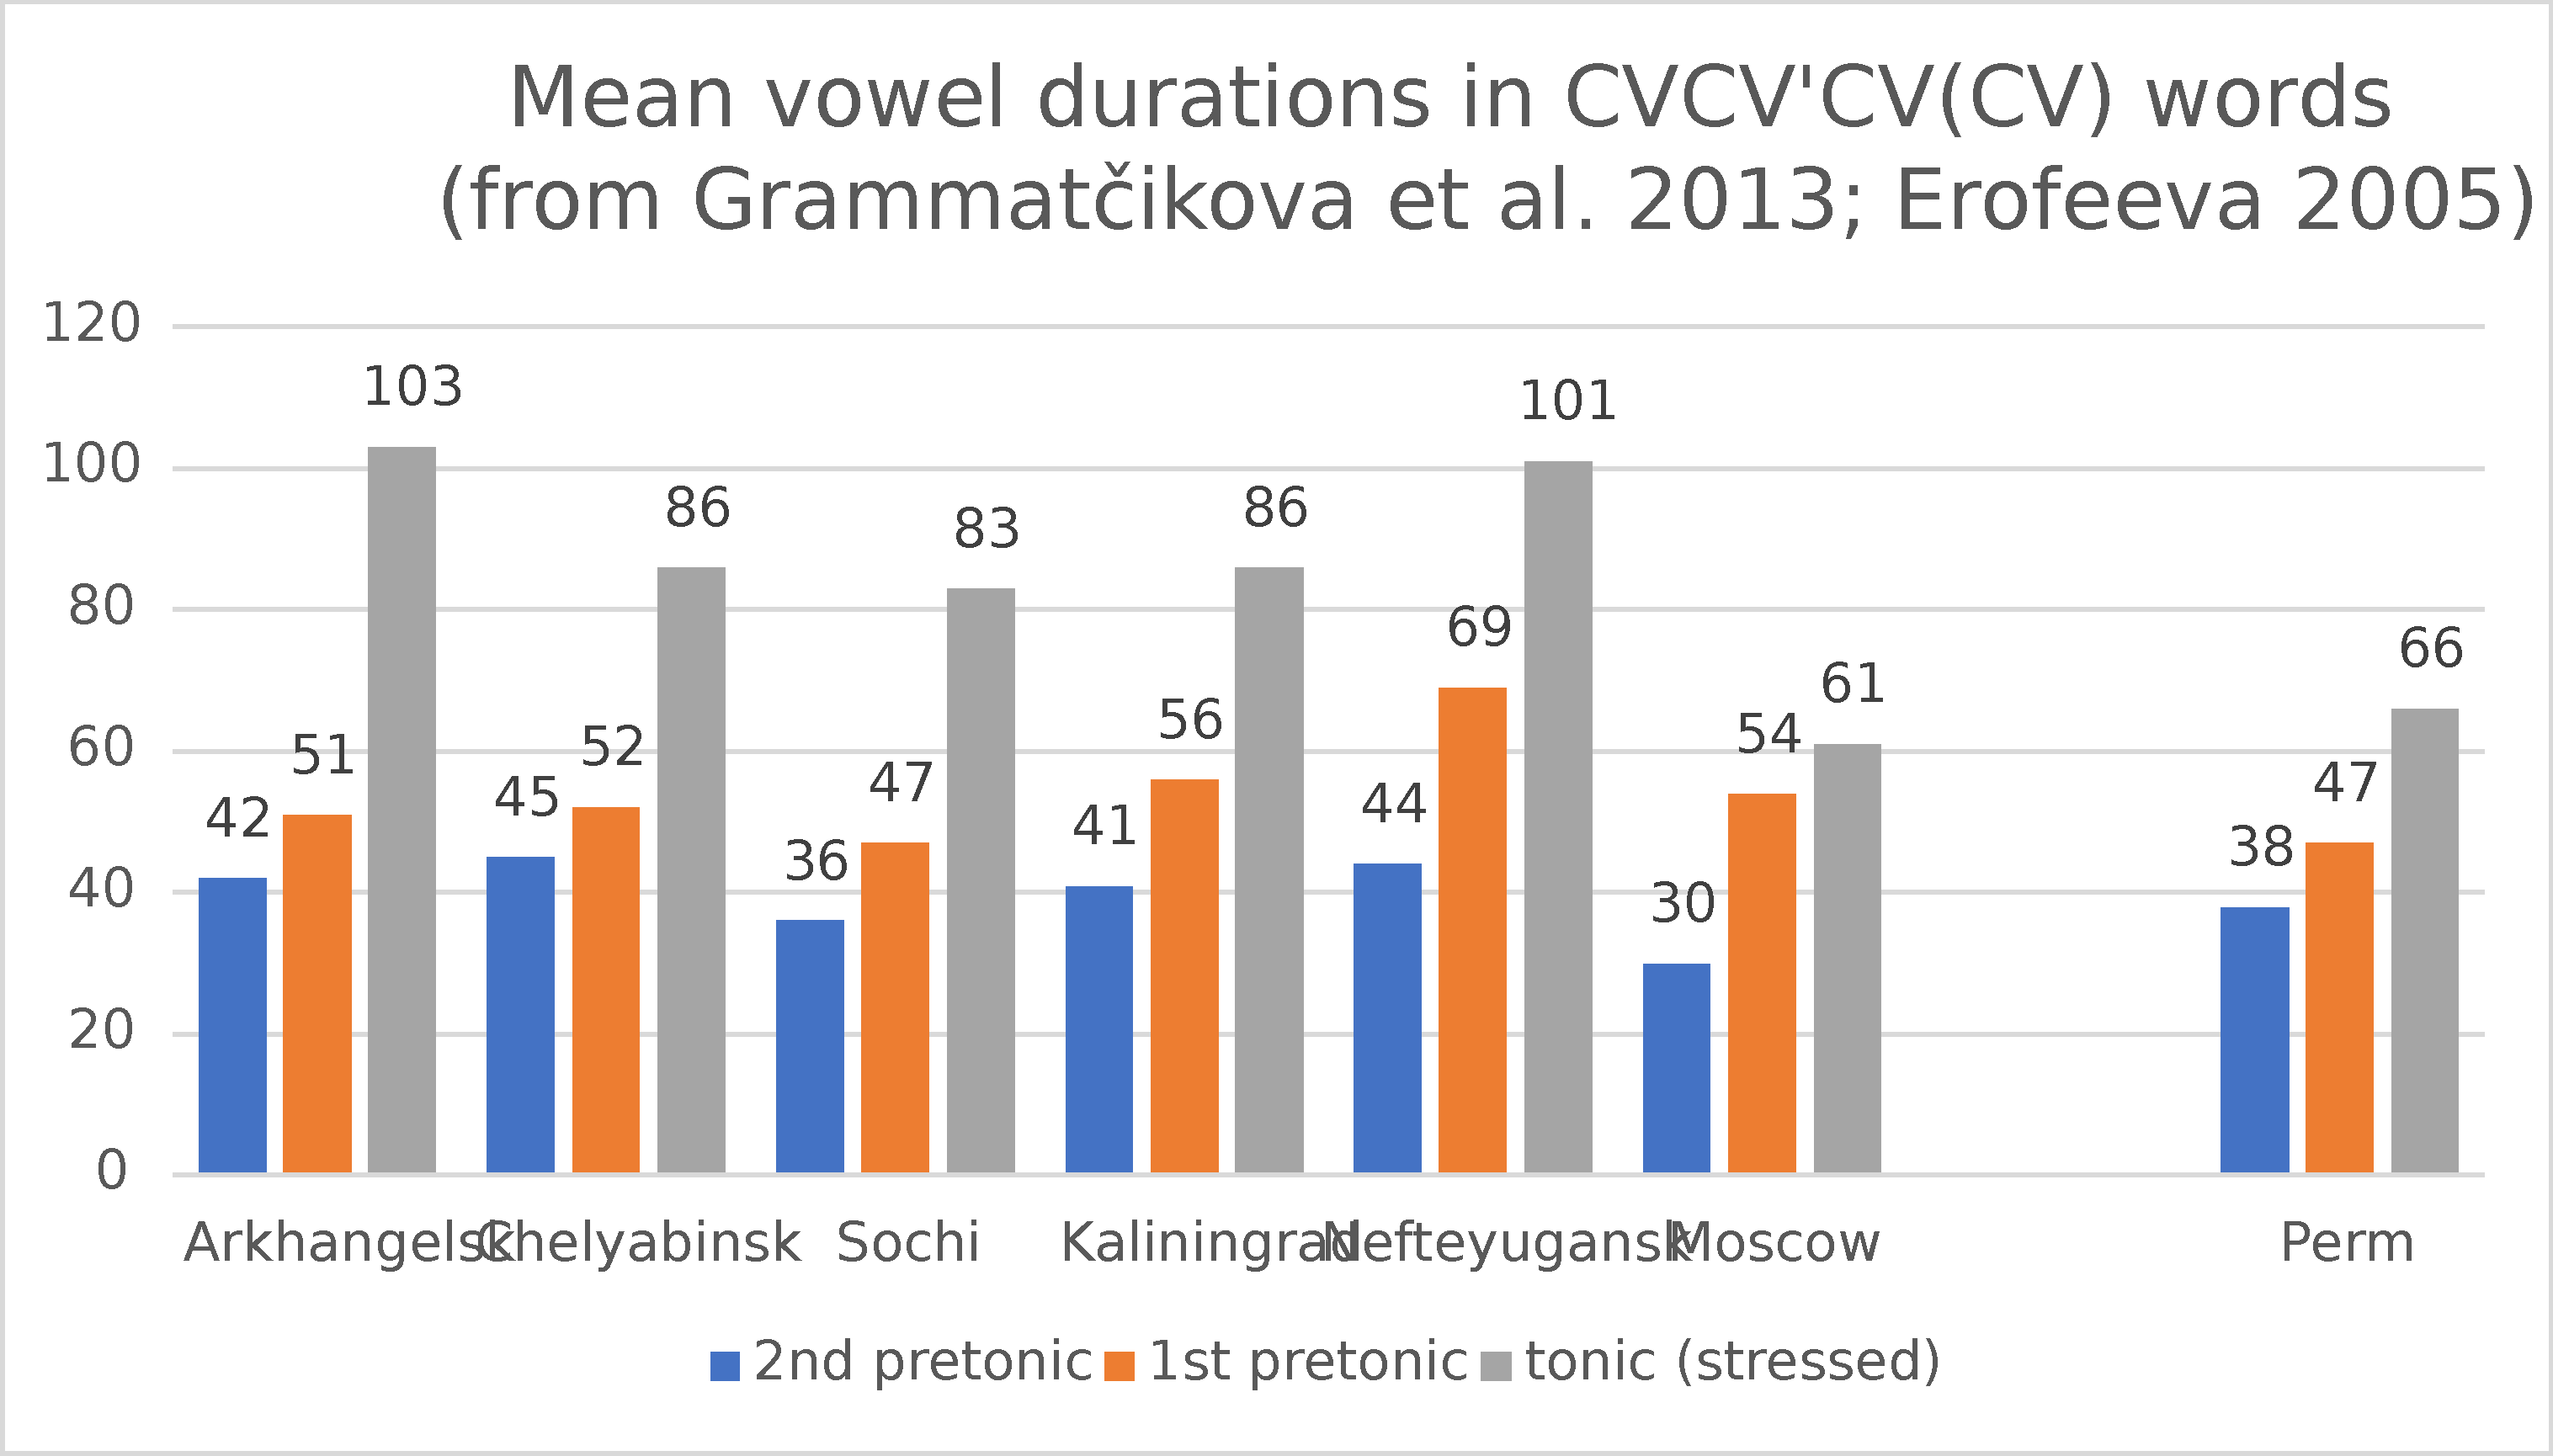
\includegraphics[width=\textwidth]{PostFig2A meanvowelgramErof_abs.pdf}
% % % 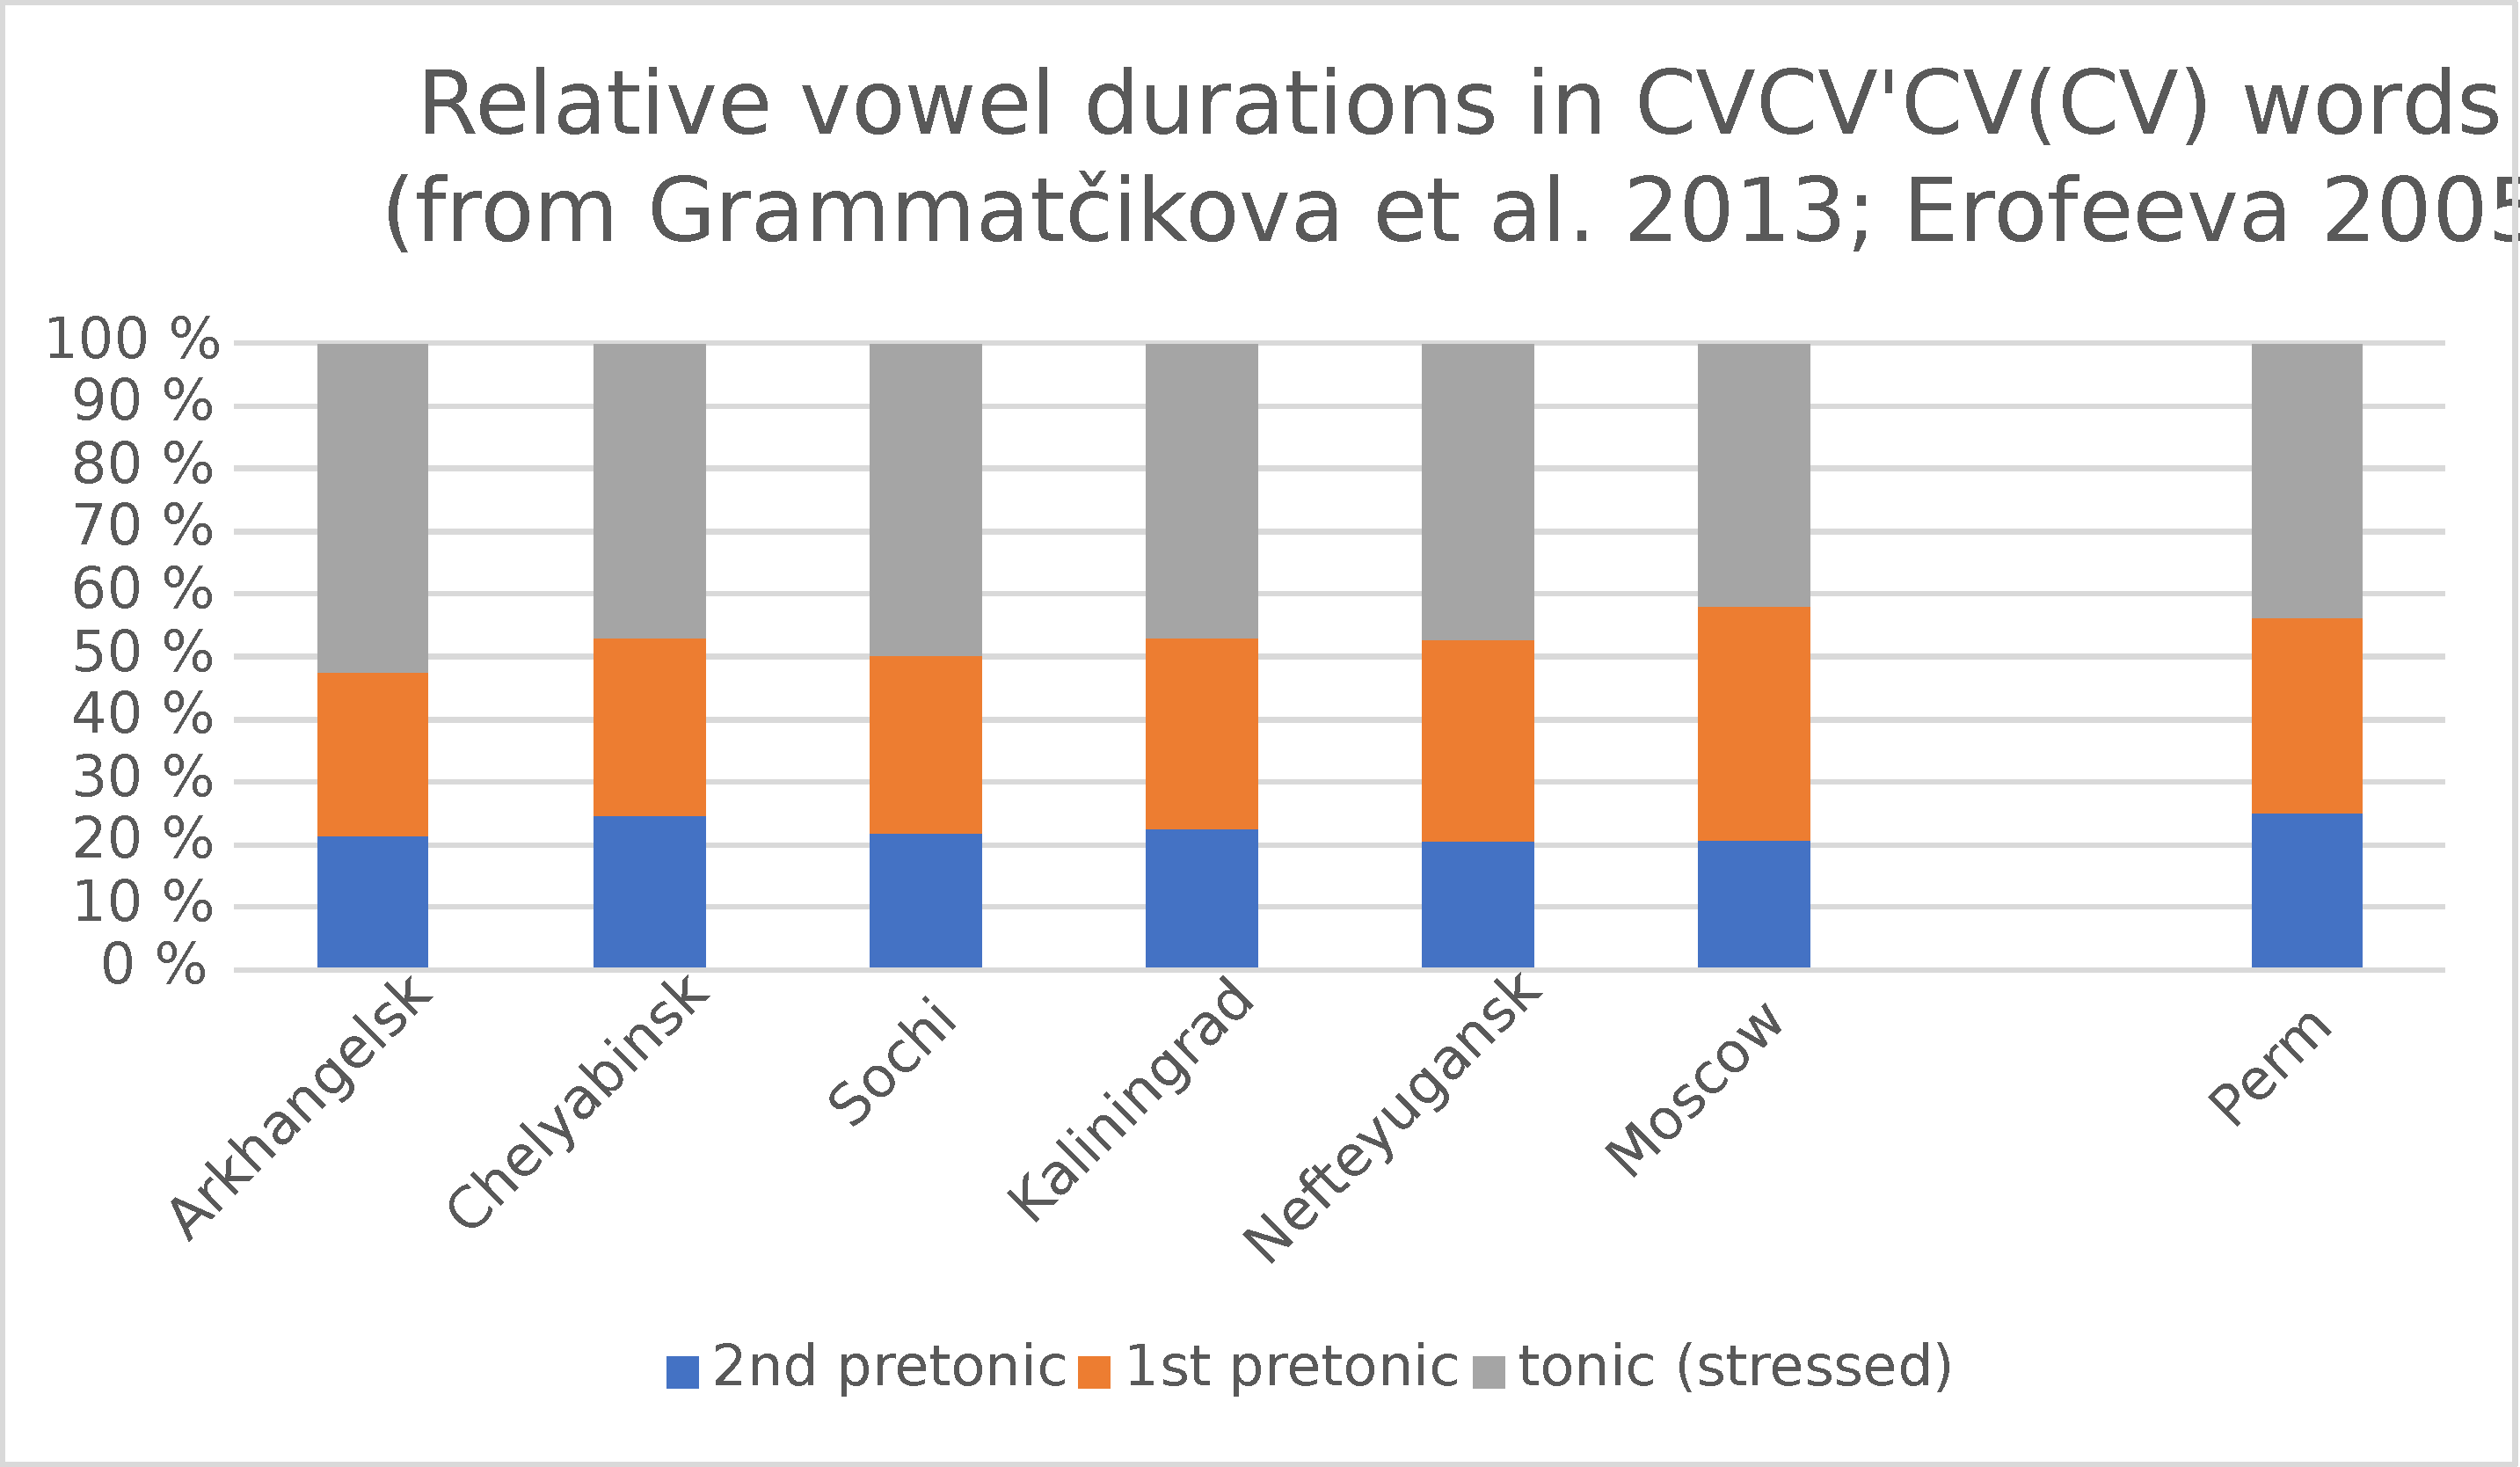
\includegraphics[width=\textwidth]{PostFig2B meanvowelgramErof_relat.pdf}
% %  Old caption
% % % % \caption{Mean vowel durations (in ms) of /o, a/ after non-palatalised plosives and fricatives in words with the structure CV-CV-ˈCVC(CV) in read speech by students from 5 cities and 1 speaker from Moscow (from \citealt{GrammatčikovaPožarickaja2013}) and in spontaneous speech by four speakers from Perm (from Appendix 1 to \citealt{Erofeeva2005}).}
\caption{Durations of /o, a/ after non-palatalised plosives and fricatives in words with the structure CV-CV-ˈCVC(CV), in read speech by students from 5 cities and one adult from Moscow (from \citealt{GrammatčikovaPožarickaja2013}) and in spontaneous speech (sp) in Perm (from Appendix 1 to \citealt{Erofeeva2005}).}
\label{fig:post:2}
\end{figure}



The small-scale study by \citet{Erofeeva2005}, of relative vowel duration of unstressed \mbox{/a/} and \mbox{/o/} in spontaneous speech by four speakers from Perm with an audible local accent, showed hardly any reduction in two degrees: The vowels in first pretonic position were only slightly longer than those in second pretonic position (\citealt{Erofeeva2005}, data from Appendix 1). In these data, /a, o/ have mean durations of 38.2 : 46.8 : 65.7 ms (for a\textsubscript{$-2$} : a\textsubscript{$-1$} : á\textsubscript{0}; $n = 308$, cf. Figure 2).



Since these two studies of regional Russian analysed only a few speakers, their data need to be confirmed using larger data sets.


\subsubsection{Sociolinguistic variables}
\label{sec:post:1.2.4}
Previous literature suggests that a lack of reduction in two degrees is not a stigmatised dialectal feature. \citet{Bondarko1998} considers the pronunciation of \mbox{/o/} as unreduced [o] in unstressed position as \textit{dialectal} (and as violating the \textit{orthoepic}, phonological rules of standard Russian), whereas pronunciation of \textit{golová} as [gʌlʌˈva] instead of normative [gəlʌˈva] -- i.e. with reduction and neutralisation, but without differentiating between two qualitative degrees of reduction -- is considered as pronunciation with an \textit{accent}, violating only \textit{orthophonic} rules, which concern the phonetic realisation of sounds \citep[249]{Bondarko1998}. Speaking with dialectal features has low social status, for in Russian, the term \textit{dialects} and \textit{dialectal} refer to traditional rural dialects, which are associated with the speech of poor, elderly villagers with little education, living in backward regions. So, avoidance of unreduced unstressed \mbox{/o/} in formal speech has higher priority than to distinguish two degrees. Furthermore, the literature only mentions the status of two-degree reduction in quality, not in quantity, suggesting that lack of a distinction in duration is even less stigmatised. The low socio-indexical status of unreduced unstressed [o] has been confirmed in attitudinal studies (e.g., in \citealt{Andrews1995}). Empirical work on vowel reduction in Perm speech shows that unreduced [o] is indeed avoided in formal speaking styles, but much less so in spontaneous speech. \citet{Erofeeva1993} found a frequency of 64\% of unreduced [o] in spontaneous speech, but only 4\% in read speech \citep{Erofeeva1993}. The same low number -- 4\% -- was also found in speech read by people from Perm in \citet{VerbickajaEtAl1984}.



Virtually no empirical studies of unstressed vowel duration appear to have been done that take sociolinguistic variables into account, but the literature suggests that the first pretonic prominence varies not only with the region, but also with age, gender, level of education and with speaking style:


\begin{itemize}
\item \textit{age}: The extra long and open first pretonic vowels in Moscow speech were common in older Moscow pronunciation (\citealt{Lapteva1999}: 354; cf. \citealt{Vysotskij1973}, group III in \figref{fig:post:1}).
\item \textit{educational level}: They are also associated more generally with vernacular Moscow speech (\citealt{Vysotskij1973}, group II; \citealt{Rozanova1988}, inter alia). 
\item \textit{gender}: Women are claimed to use extra long and prominent (in tone) first pretonic open vowels to a larger degree than men, specifically as a means for expressing emphasis, where men would typically prefer longer consonants (\citealt{ZemskajaEtAl1987, Rozanova1988, Kasatkina2003}, all based on speakers from Moscow), though \citealt{Kasatkina2005} found an equal amount of prominent first pretonic vowels among women and men in her small empirical study. In other languages, women tend to have longer vowel durations than men and in many studies, they also speak at a slower rate (e.g. \citealt{SimpsonEricsdotter2003}). Urban women also tend to use standard and other prestige forms more often than men \citep{Labov2001}.
\item \textit{speaking style}: We can expect regional differences to be lowest in a formal speaking style, such as in the reading tasks most experimental studies have been based on. In formal speech, people are more likely to adapt to standard language and suppress low-status socio-indexical features; cf. the differences in vowel quality relative to speaking style in \citet{Erofeeva1993}.
\end{itemize}

\subsection{Research questions: Moscow vs. Perm}
\label{sec:post:1.3}
Our overarching research question was whether we will find regional variation in prosody in today’s Russian urban speech. We chose to compare speakers from two large cities, Moscow and Perm. Moscow is Russia’s capital, and Moscow’s speech, especially vernacular speech, is known for long and open realisations of \mbox{/o/} and \mbox{/a/} in first pretonic position, as in [maːˈskva]. The city of Perm is situated in the Ural region on the border between European Russia and Siberia. Its speech is known for a relatively strong local accent with northern Russian traits. It is well-studied by the sociolinguists of Perm University, using probabilistic measures to study the social stratification of dialect features across speaker groups in Perm (\citealt{Erofeeva1995, Erofeeva2005}, inter alia).
%use short vertical strokes in transcriptions to indicate stress not apostrophes


More specifically, I wanted to answer the following questions:


\begin{enumerate}
\item
Two-degree reduction: How is the durational two-degree reduction expressed in the two cities? In other words, how different in duration are the two pretonic vowels from each other, and from the tonic (stressed) vowel? We expect the first pretonic vowel to be relatively longer in Moscow speech.
\end{enumerate}

This is our major question, but we also addressed possible gender effects: 


\begin{enumerate}[resume]
\item 
Gender effect on overall vowel duration: Do the female speakers have longer vowel durations than the male speakers, in both cities?

\item 
Gender effect on duration of the first pretonic vowel: Do the girls use extra prominence on the first pretonic vowels, measured in duration, more often than the boys?

\item Gender effect on relative distance in vowel duration between the two cities: Do the Perm girls have a reduction pattern closer to that of the Moscow speakers, with stronger two-degree reduction, than the boys? If it is true that girls tend to converge more to standard language – or to another non-local norm with high status – also in Russian, then we can expect to see smaller differences between the female speakers than between their male peers from Moscow and Perm.
\end{enumerate}

\section{Data and methods}
\label{sec:post:2}
\subsection{Materials}
\label{sec:post:2.1}
We asked participants in both cities to read aloud an utterance list containing trisyllabic words with final stress. The three target words in the reading task were \mbox{/potaˈkatʲ/} `to connive', /topoˈtatʲ/ `to stamp feet' and /pokoˈpatʲ/ `to dig a little', three words that were also analysed in \citet{Vysotskij1973}. They contain \mbox{/a/} and \mbox{/o/} after the non-palatalised voiceless plosives /p, t, k/, which facilitate vowel segmentation, and have the rhythmic structure CV-CV-ˈCVC. I will call the vowels in second pretonic position a\textsubscript{$-2$}, the first pretonics a\textsubscript{$-1$} and the tonic (stressed) vowels á\textsubscript{0}. The symbols a\textsubscript{$-2$} and a\textsubscript{$-1$} stand for the phonemes \mbox{/a/} and \mbox{/o/}, which merge in unstressed position in Standard Russian.



We analysed 6 sentences, covering each word in two prosodic conditions: in utterance-medial position carrying the nuclear (final) accent, represented by \REF{ex:post:1} below, and in utterance-medial prenuclear position \REF{ex:post:2}:\footnote{We recorded a larger number of utterances and more speakers – 10 utterances by 33 speakers, but we had gaps in the data due to misreadings, some clear cases of unnatural speech, long hesitations or pauses, or creaky voice. For the Moscow speakers, discarded renderings could be replaced by their second renderings. This could not be done for the Perm speakers, who read the utterances only once. We also discarded all data from one male speaker from Perm, because of disfluent speech, and from one female speaker from Perm, because of creaky voice. In order to avoid gaps in the data, we excluded several more speakers and the first renderings of the words (in citation form), which were sometimes read with hesitation, because some of the speakers might not have been familiar with the uncommon target words \textit{topotat'} and \textit{potakat'}. This left us with 26 speakers reading 6 utterances each (\tabref{tab:post:1}).}

\ea \label{ex:post:1}
utterance-medial, nuclear position:\\
\gll \textit{Ja}        \textit{pokopát'}  \textit{pošla.}\\
     \textsc{I}.\textsc{nom} dig.\textsc{inf}       go-\textsc{f.sg.pst}\\
\glt `I went digging.'
\z 

\ea \label{ex:post:2}
utterance-medial, prenuclear position: \\
\gll \textit{Ja}       \textit{topotát’}   \textit{uže}        \textit{ne}   \textit{budu.}\\
     \textsc{I}.\textsc{nom} patter.\textsc{inf} already \textsc{neg} \textsc{1sg.ipfv.fut}\\
\glt `I won’t patter anymore.'\\
\z

\begin{sloppypar}
We left out utterance-initial and utterance-final positions in order to avoid boundary phenomena, which typically affect duration -- utterance-initial strengthening and final lengthening.
\end{sloppypar}



The reading task was performed in 2015 by 15--17-year-old pupils at a school in Perm and a school in Moscow, who were born in these cities or had moved there before the age of 6. Almost all speakers have parents with higher education. We have not screened our participants and assessed to which degree they speak with a local accent. Therefore, one cannot equate the speech of our Moscow participants with Central Standard Russian, but since the recordings are made in a formal setting and most pupils in both cities have parents with higher education, a strong degree of local vernacular accent is unlikely.



Six utterances each by 13 female and 13 male speakers were analysed for the present study (\tabref{tab:post:1}). The same speakers performed a range of other tasks (reading, semi-spontaneous and spontaneous speech and interviews), collected for, or in association with, Benedikte Vardøys PhD project on young Russians’ perception of regional variation in Russian (cf. \citealt{Vardøy2021, RN1173}). The sound recordings were made in the school library or in a small room, using digital recorders and unidirectional head-mounted microphones (a Zoom H5 recorder with a Shure WH20 microphone in Perm, a Zoom H2 with a Samson QV mic in Moscow, set at 44.1 kHz, 16-bit, .wav). The participants read the utterances from paper, in the same order, a single time in Perm, two times in Moscow.


\begin{table}
\begin{tabular}{lrrrrr}
\lsptoprule
 & {speakers} & { F} & { M} & { word tokens} & {vowel tokens}\\
\midrule
 Moscow &  13 &  7 &  6 &  78 &  234\\
Perm &  13 &  6 &  7 &  78 &  234\\
Total &  26 &  13 &  13 &  156 & 468\\
\lspbottomrule
\end{tabular}
\caption{\label{tab:post:1}Number of speakers and tokens analysed for the present study}
\end{table}

\subsection{Acoustic and statistical analyses}
\label{sec:post:2.2}
The target vowels in the speech samples were manually segmented in Praat (\citealt{BoersmaWeenink1992}) via visual inspection of the waveform and spectrogram according to standard segmentation criteria; for examples, see \figref{fig:post:3} and \figref{fig:post:4}. The durations of the target vowels per speaker and location were extracted using Praat scripts.


\begin{figure}
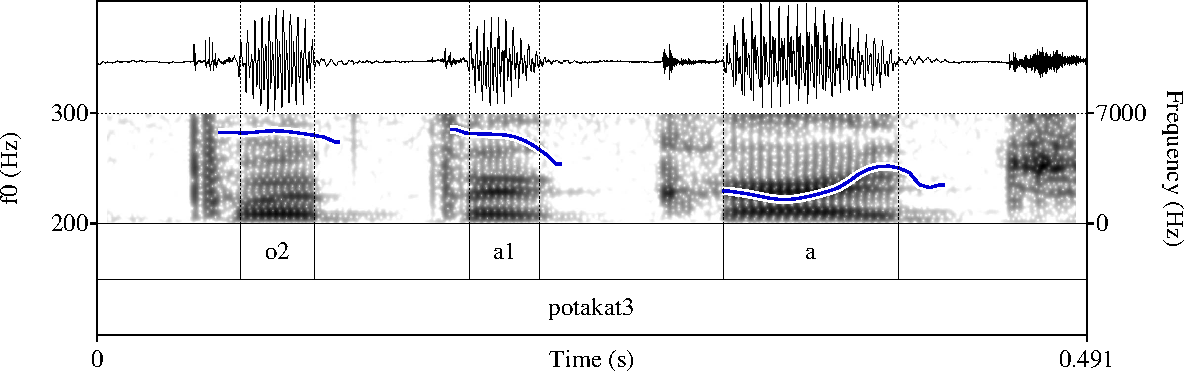
\includegraphics[width=\textwidth]{PostFig3_390F_potakat3-w-ps-t.pdf}
\caption{\label{fig:post:3} Waveform, spectrogram and F0 contour, with segmented vowels, of the target word \textit{potakát’}, produced by a female speaker from Perm (ID 390F), made in \textit{Praat} \citealt{BoersmaWeenink1992}}
\end{figure}



\begin{figure}
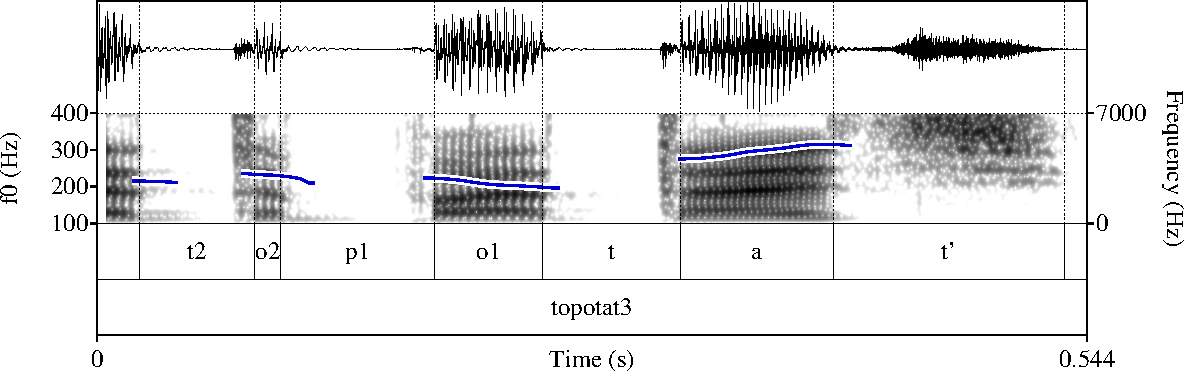
\includegraphics[width=\textwidth]{PostFig4_Mo15_10F_topotat3_cons-w-ps-t.pdf}
\caption{\label{fig:post:4} Waveform, spectrogram and F0 contour, with segmented vowels and consonants, of the target word \textit{pokopát’} in utterance \REF{ex:post:2}, produced by a female speaker from Moscow (ID 10F)}
\end{figure}


For statistical validation, we used the software JMP 16.2.0. Vowel durations were log-transformed because of positive skewness. As a first step towards determining the differences, linear mixed models (LMM) were fitted with the respective log-transformed measure as dependent variable and \textsc{distance-to-stress} with three factor levels (0/1/2), \textsc{location} with two factor levels (Moscow/Perm) and \textsc{gender} with two factor levels (male/female) as fixed factors, as well as all their possible interactions. \textsc{speaker}, \textsc{word} (\textit{topotát’}/\textit{pokopát’}/\textit{pokatát’}) and \textsc{position-in-utterance} (utterance-medial prenuclear\slash utterance-medial nuclear accent) were taken as random factors. Separate post-hoc tests were carried out per variable, if appropriate. The confidence level was set at $\alpha = 0.05$.


\section{Results}
\label{sec:post:3}
Predictably, we found a main effect of \textsc{gender} (F [1, 22] = 4.1169, $p < 0.05$) and of \textsc{distance-to-stress} (F [2, 431] = 815.4856, $p < 0.001$) on the target vowel duration, with female speakers having significantly longer durations (cf. \figref{fig:post:5}, female voices in blue), and stressed vowels (á\textsubscript{0}) being longer than the vowels in the first pretonic syllable (a\textsubscript{$-1$}), which in turn are longer than the vowels in the second pretonic syllable (a\textsubscript{$-2$}), when taking both cities together \citep{postaccepted}. The variable \textsc{location} (F [1, 22] = 4.1169, $p = 0.055$) was not significant.


\begin{figure}
% % % 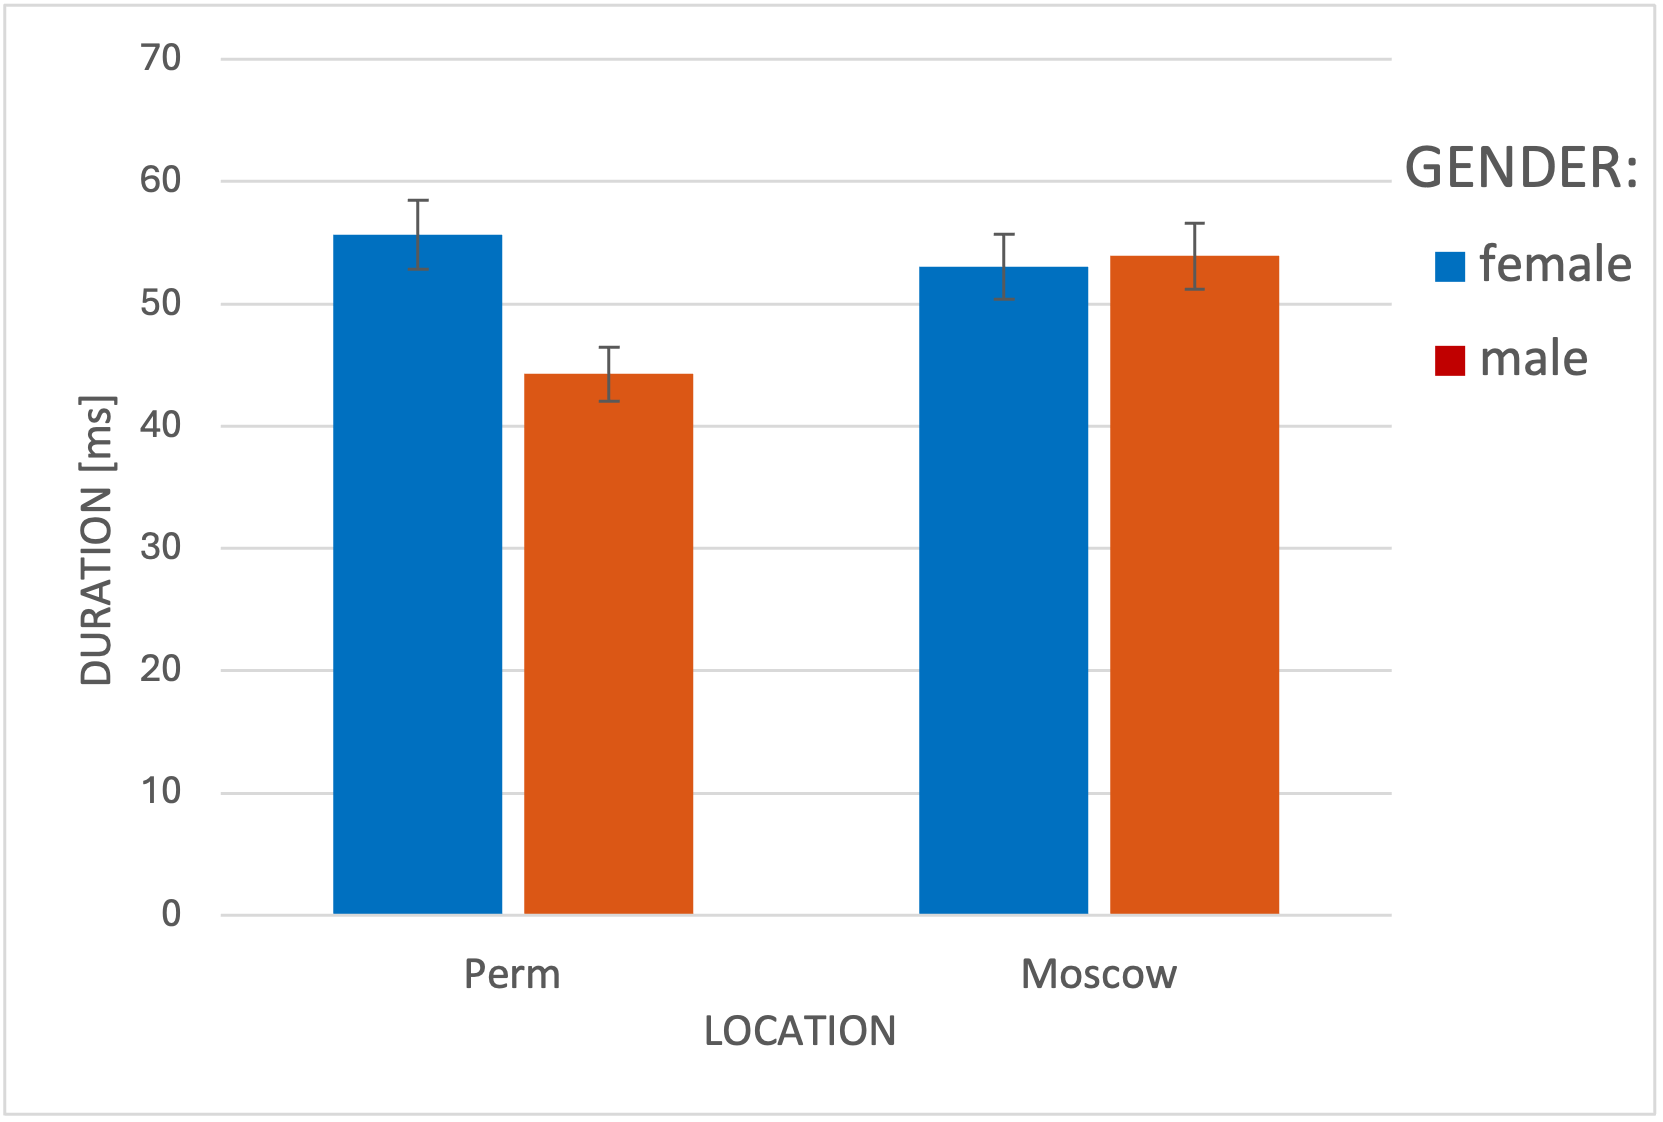
\includegraphics[width=\textwidth]{PostFig5_Location-Gender.png}\\
\begin{tikzpicture}
\small
\begin{axis}
	[
        axis lines*=left,
		bar width=4ex,
		font=\small,
		height=5cm,
		enlarge x limits=0.50,
		legend cell align=left,
		legend pos = outer north east,
		width=.5\textwidth,
		xtick=data,
		symbolic x coords={Perm,Moscow},
        ybar=2*\pgflinewidth,
		ylabel={Duration (ms)},
		xlabel=Location,
		ylabel near ticks,
		ymin=0,
		ymajorgrids=true
	]
	\addlegendimage{empty legend}
	\addlegendentry{Gender}
	\addplot+ [style={lsDarkBlue,fill=lsMidBlue}, error bars/.cd, y dir=both, y explicit] 
	  coordinates{(Perm,55.7) +- (3.1201,3.1201) (Moscow,53.1) +- (2.4,2.4)};
	\addlegendentry{Female}
	\addplot+ [style={lsRed,fill=lsDarkOrange}, error bars/.cd, y dir=both, y explicit] 
	  coordinates{(Perm,44.3) +-(2.5458,2.5458) (Moscow,53.9) +- (2.6586,2.6586)};
	\addlegendentry{Male}
\end{axis}
\end{tikzpicture}
\caption{\label{fig:post:5}\textsc{location} vs. \textsc{gender}: Mean duration of vowels (all three positions together), for Perm (left) and Moscow (right), with female speakers in blue and male speakers in red. Error bars represent standard errors.}
\end{figure}


The statistical analysis also revealed a significant interaction between \textsc{location} and \textsc{gender} (F [1, 22] = 8.4120, $p < 0.01$). Post-hoc tests revealed that the girls from Perm have significantly longer vowels than their male classmates, but in Moscow, the girls and boys have similar vowel durations (see \figref{fig:post:5}). This means that the earlier mentioned gender effect is only found in Perm.



More relevant for our main research question is the highly significant interaction between \textsc{location} and \textsc{distance-to-stress} (F [2, 431] = 65.0217, $p < 0.001$). In the realisations of the speakers from Moscow, vowel durations become significantly shorter with increasing distance from the stressed syllable, whereas in the realisations of the speakers from Perm, the vowels in the stressed syllable are significantly longer than the vowels in both first and second pretonic syllable (\figref{fig:post:6}). When comparing the mean values of actual durations according to positions to stress in \figref{fig:post:6}, we see that in Moscow, the vowels in the first pretonic position are, on average, twice as long as the vowels in the second pretonics, for both male and female speakers. In Moscow, the relative durations of the three consecutive vowels (a\textsubscript{$-2$} : a\textsubscript{$-1$} : á\textsubscript{0}) are almost 1 : 2 : 3 (with actual values 24.1 ms : 49.5 ms : 82.8 ms). In Perm, the difference between the two prestressed vowels is surprisingly small, the ratio being almost 1 : 1 : 3 (with the actual values 28.3 ms : 33.1 ms : 89.3 ms). The letter report from the post-hoc pairwise Tukey HSD test of the mean durations (log-transformed; \tabref{tab:post:2}) shows that the small difference in duration between the pretonic vowels in Perm is not statistically significant, since a\textsubscript{$-2$} and a\textsubscript{$-1$} in Perm share the letter \textit{C}, whereas a\textsubscript{$-2$} and a\textsubscript{$-1$} in Moscow end up with the letters \textit{B} and \textit{D}, respectively (\tabref{tab:post:2}).



\begin{figure}
% % % 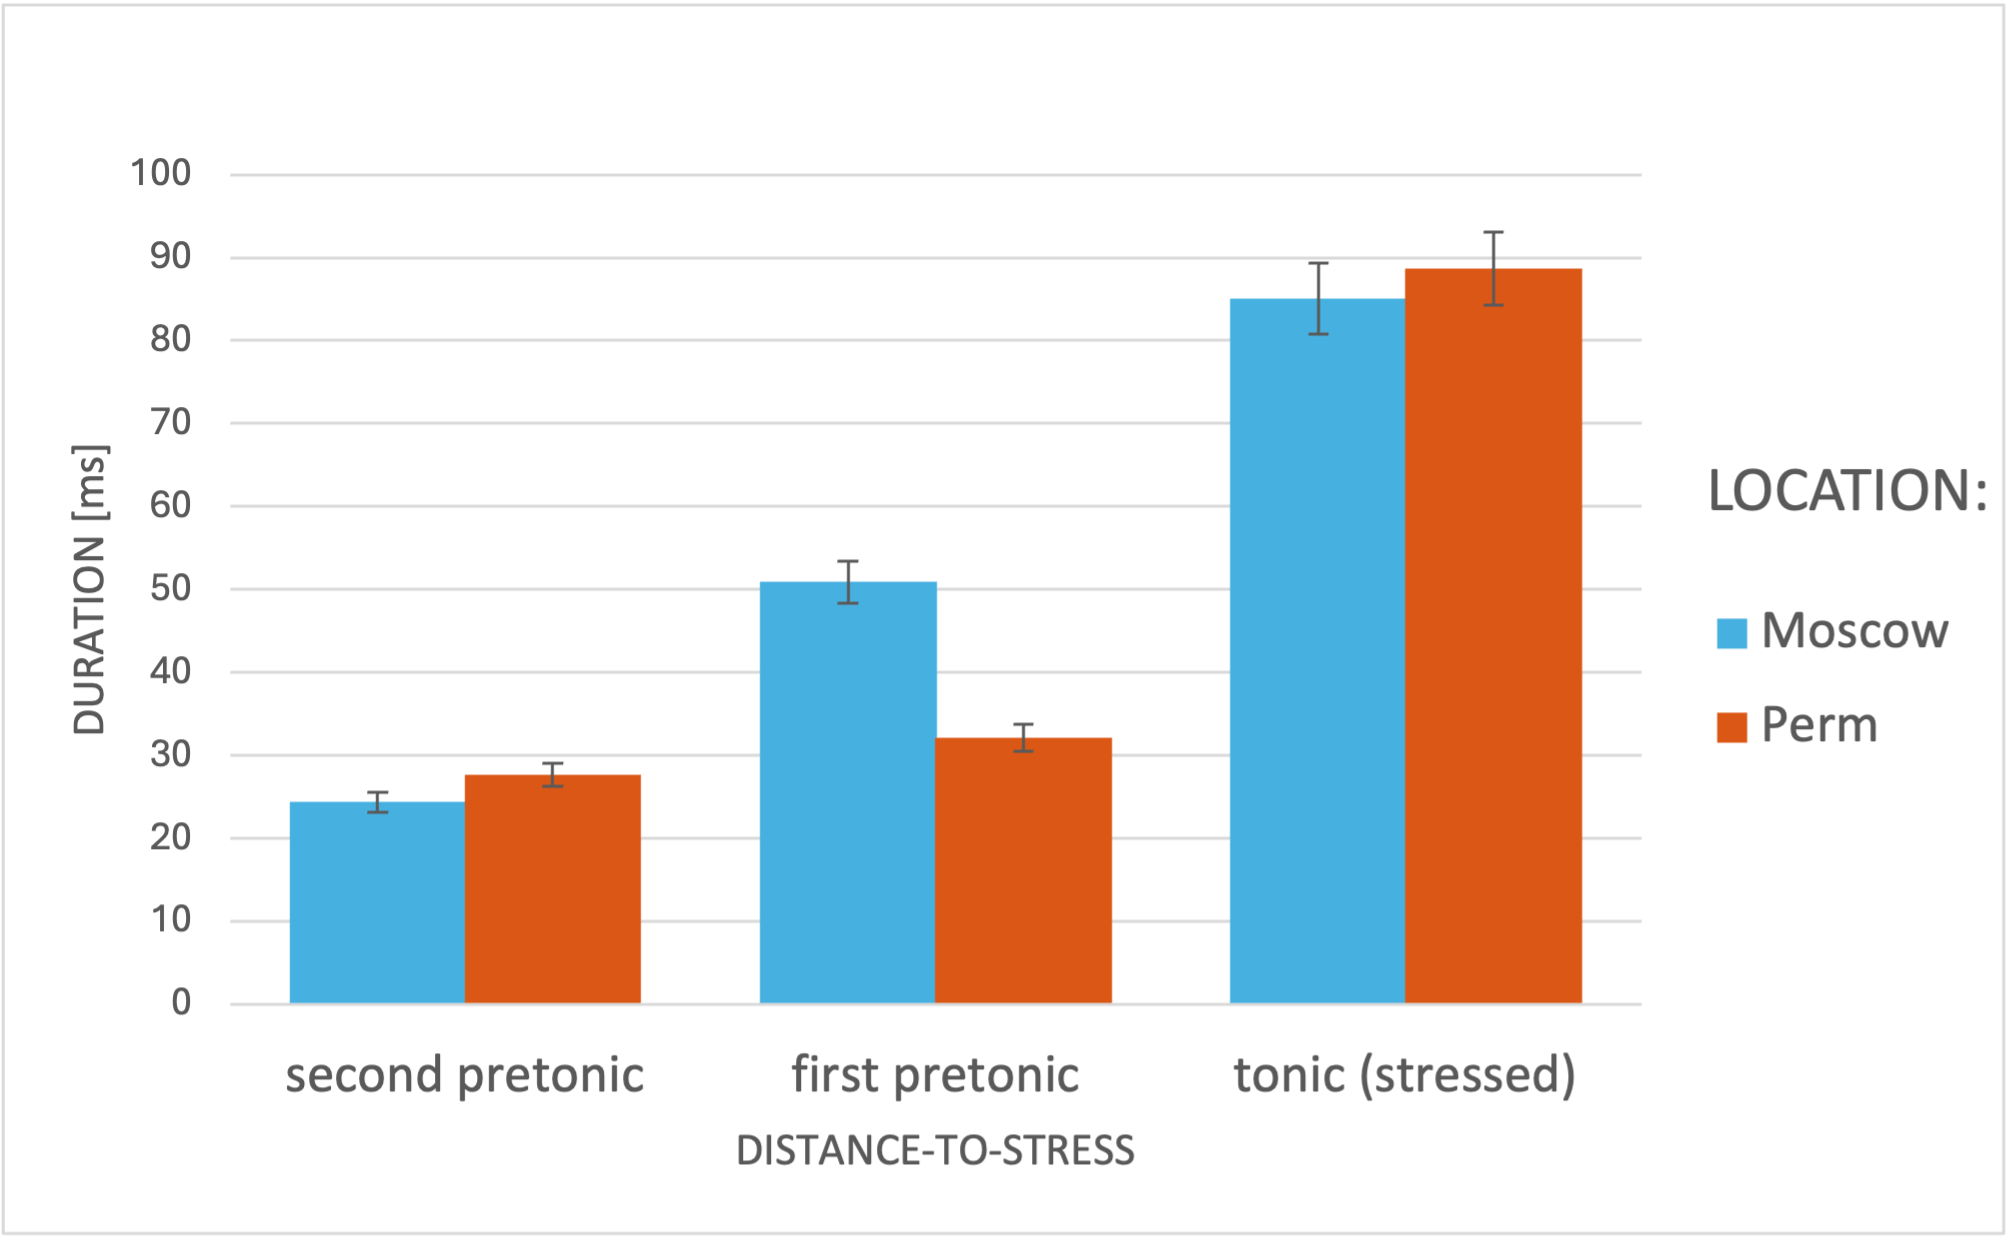
\includegraphics[width=\textwidth]{PostFig6_distance_to_stress_location.png}
\begin{tikzpicture}
\small
\begin{axis}
	[
        axis lines*=left,
		bar width=4ex,
		font=\small,
		height=5cm,
		enlarge x limits=0.50,
		legend cell align=left,
		legend pos = outer north east,
		width=.8\textwidth,
		xtick=data,
		symbolic x coords={second pretonic,first pretonic,{tonic (stressed)}},
        ybar=2*\pgflinewidth,
		ylabel={Duration (ms)},
		xlabel={Distance-to-stress},
		x tick label style={text width=1.5cm, align=center},
		ylabel near ticks,
		ymin=0,
		ymajorgrids=true
	]
	\addlegendimage{empty legend}
	\addlegendentry{Location}
	\addplot+ [style={lsDarkBlue,fill=lsMidBlue}, error bars/.cd, y dir=both, y explicit]
	  coordinates{(second pretonic,24.4) +-(0.942,0.942) (first pretonic,50.9) +-(0.9468,0.9468) ({tonic (stressed)},85.1) +- (1.6952,1.6952)};
	\addlegendentry{Moscow}
	\addplot+ [style={lsRed,fill=lsDarkOrange}, error bars/.cd, y dir=both, y explicit]
	  coordinates{(second pretonic,27.7) +- (1.0454,1.0454) (first pretonic,32.2) +-(1.3382,1.3382) ({tonic (stressed)},88.7) +- (2.0047,2.0047)};
	\addlegendentry{Perm}
\end{axis}
\end{tikzpicture}
\caption{\label{fig:post:6}\textsc{location} vs. \textsc{distance-to-stress:} Mean duration according to distance-to-stress and location (blue = Moscow; red = Perm; both genders). Error bars represent standard errors.}
\end{figure}

\begin{table}
\begin{tabular}{lccccr}
\lsptoprule
{ Level} &  &  &  &  & Least Sq Mean\\
\midrule
P, tonic & A &  & ~ & ~ & 4.4715085 \\
M, tonic & A &  & ~ & ~ & 4.4284267 \\
M, 1st pretonic &  & B & ~ & ~ & 3.9156951 \\
P, 1st pretonic &  & ~ & C & ~ & 3.4001192 \\
P, 2nd pretonic &  & ~ & C & D & 3.2752833 \\
M, 2nd pretonic &  & ~ & ~ & D & 3.1268467 \\
\lspbottomrule
\end{tabular}
\caption{\label{tab:post:2} Connected Letter report from pairwise Tukey HSD test of mean durations (log-transformed), according to location and distance-to-stress. Levels not connected by the same letter are significantly different.}
\end{table}

We saw that the female speakers use longer vowels than the men (in Perm), but the relative durations are not affected by gender: There was no significant interaction between \textsc{gender} and \textsc{distance-to-stress} (F [2, 431] = 1.3204, $p > 0.05$), nor between all three variables \textsc{location,} \textsc{distance-to-stress} and \textsc{gender} together (F [2, 431] = 1.4552, $p > 0.05$). The girls use the same vowel rhythm as the boys in each city: In Moscow, the relative durations of a\textsubscript{$-2$} : a\textsubscript{$-1$} : á\textsubscript{0} are 15 : 32 : 53\% (of the total vowel duration in the word) for the girls and 15 : 31 : 53\% for the boys; in Perm, the numbers are 19 : 22 : 58\% for the girls and 18 : 21 : 61\% for the boys. 



One must take into account that these numbers are mean values and that the variation between individual tokens is large. However, even with this large degree of variation, the difference between Moscow and Perm is highly significant.



When comparing the mean durational values of each individual speaker, one can see that all 13 speakers in Moscow had a larger durational difference between the two prestressed vowels than all 13 speakers in Perm. This result suggests that not a single speaker in Perm uses a Moscow word rhythm, or the other way round.



When we look even closer at all individual word tokens in Moscow, the second pretonic vowel is shorter than the first pretonic in all but a single case -- in 77 out of 78 word tokens. In Perm, it is shorter in only 51 out of 78 renditions. This suggests that the two-degree reduction is very stable in Moscow.


\section{Discussion}
\label{sec:post:4}
\subsection{Large difference between pretonic vowels in Moscow, not in Perm}
\label{sec:post:4.1}
Our main research question concerns the expression of reduction in two degrees, that is, the relative durations of the second and first pretonic vowels (research question 1). As expected, we found a larger difference in duration between the two pretonic positions in Moscow than in Perm. This correlation between location and distance to stress is stronger than expected. The difference between the cities is not only large, but also stable, since all Moscow speakers have a rhythm different from all Perm speakers. 



In Moscow, the distinction between the two vowels is very robust: not only is a\textsubscript{$-1$} on average twice as long as a\textsubscript{$-2$} (\figref{fig:post:6}), it is also longer in all but one word production in Moscow. Mark that a\textsubscript{$-1$} would have been even longer in the position preceding a high vowel, since Moscow has clear vowel dissimilation in duration (\citealt{Kasatkina2005}, cf. \sectref{sec:post:1.2.3} above). Obviously, the reduction in two degrees is categorical for the Moscow speakers. A study of the formant values of our data shows that the large difference in duration between the two pretonic positions is paralleled by a large difference in first formant values \citep{postaccepted}, confirming that our Moscow speakers use reduction in two degrees in both quantity and quality. In Perm, on the other hand, we see huge variation and no statistically significant average durational difference between a\textsubscript{$-1$} and a\textsubscript{$-2$}, suggesting it is not a categorical distinction in Perm speech.



When comparing our data with previous research, we find that the Moscow durational pattern of almost 1 : 2 : 3 for a\textsubscript{$-2$} : a\textsubscript{$-1$} : á\textsubscript{0} is actually very close to Potebnja’s formula for standard Russian vowel strength, and the relative durations \citet{Bondarko1998} refers to, although other studies of CSR found smaller (e.g. \citealt{Vysotskij1973}, group I) or larger differences (e.g. \citealt{Barnes2006}) between the two pretonic positions. Our results from Moscow of almost 1 : 2 : 3 range between Vysotskij’s group I for standard pronunciation (58 : 80 : 118 ms) and group II for Moscow vernacular speech (35 : 92 : 113 ms; \figref{fig:post:1}, groups I and II).\footnote{Our data are not fully comparable to the results from previous studies, since not all parameters influencing vowel duration always coincide. For instance, \citet{Vysotskij1973} included words in utterance-final position. Still, most previous research is based on words with very similar segmental and rhythmic structure as the current study.}


\begin{sloppypar}
As a possible reference example of CSR pronunciation, I also recorded a teacher of Russian as a foreign language, who was born in Leningrad (Saint Petersburg) in the 1950s but has lived most of her life in Moscow. Her mean durations of a\textsubscript{$-2$} : a\textsubscript{$-1$} : á\textsubscript{0} were 35.8 : 83.6 : 126.5 ms (cf. \figref{fig:post:7} below), so her values are closer to Vysotskij’s measurements from Moscow vernacular speech than to his values for CSR and to our data from Moscow adolescents.
\end{sloppypar}



We have not assessed to which degree our adolescent speakers in Moscow and Perm speak standard Russian, with or without local colouring. We can conclude that the Moscow boys and girls have weaker local colouring in their word rhythmic pattern than the older teacher, but their difference between degree 1 and degree 2 reduction is larger than in most existing data for Central Standard Russian. 



Our Perm pattern of almost 1 : 1 : 3, with only a small durational difference between the unstressed vowels (a\textsubscript{$-2$} is, on average, 86\% of a\textsubscript{$-1$}), is not the closest to Vysotskij’s dialect group represented in the Ural region (\figref{fig:post:1}, group IX), as one could expect, since Perm is situated there. This group has a larger difference between the two pretonic vowels (with 33 : 53 : 78 ms for a\textsubscript{$-2$} : a\textsubscript{$-1$} : á\textsubscript{0}). Our Perm rhythm is actually closest to dialect group VIII, the rural dialect system with the smallest difference between a\textsubscript{$-2$} and a\textsubscript{$-1$}, found in a peripheral area in the North of European Russia (\figref{fig:post:1}, group VIII, where a\textsubscript{$-2$} is 90\% of a\textsubscript{$-1$}). The two-degree reduction in Perm is also less pronounced than in the data from Arkhangelsk and Chelyabinsk (\figref{fig:post:2}), the two students with the smallest difference in \citegen{GrammatčikovaPožarickaja2013} study of modern regional standard speech. In our data from Perm, the a\textsubscript{$-2$} : a\textsubscript{$-1$} ratio is similar to the ratio in \citegen{Erofeeva2005} data from 4 speakers with a Perm accent, with 0.87 : 1 resp. 0.81 : 1. An important difference between our and Erofeeva’s data is that the latter are from spontaneous speech; cf. \sectref{sec:post:4.4.3} below. One of the pupils we recorded in Moscow happened to be from the Northern Vologda region. He, too, made hardly any difference between a\textsubscript{$-2$} and a\textsubscript{$-1$}, although all his vowels had longer durations than his peers in Moscow and Perm (40 : 44 : 94 ms; represented as V in \figref{fig:post:7} in the next section). One should be aware that these single speakers from our own data, as well as those from earlier literature, need not be representative of the word rhythm of the city where they grew up, but they probably give some indication of it, since our data from Moscow and Perm suggest that word rhythm is a relatively stable regional trait.



When comparing the first pretonic vowel a\textsubscript{$-1$} with the stressed vowel a\textsubscript{0}, the stressed vowel is much longer than both prestressed vowels in our data, both in Perm and in Moscow. The difference between a\textsubscript{$-1$} and\textsubscript{} a\textsubscript{0} is smaller in \citegen{Erofeeva2005} data from Perm and considerably smaller in most studies of CSR (e.g., \citealt{Knjazev2006, GrammatčikovaPožarickaja2013}).\footnote{An exception, with a large difference between a\textsubscript{$-1$} and\textsubscript{} a\textsubscript{0}, is \citegen{Duryagin2018} speaker of CSR, whose vowel durations were 37 : 60 : 106 ms \citep[327]{Duryagin2018}, but here, the difference is partly caused by the words' utterance-final position, which can cause final lengthening.} This is mainly due to the uncommonly short pretonic vowels among our adolescent speakers. Perm and Moscow show little difference in their relative duration of the stressed vowel. This might be a general feature of varieties of Russian. The data in \figref{fig:post:1} from \citet{Vysotskij1973} show considerable variation between the varieties in the first and second pretonic vowel, but a remarkably stable relative duration of the stressed vowel, of almost 50\% of the total duration of all three vowels in all 6 represented rhythmic patterns. In our data, the relative duration of the tonic vowel is not very different, though somewhat longer: 51\% in Moscow and 58\% in Perm. Vysotskij included target words in utterance-final position, which may have led to relatively longer stressed vowels and thus a larger proportion of the total than in our data with only non-utterance-final positions. Still, the last vowel had a relatively longer duration in our data.


\subsection{First pretonic prominence is relative: Vowels vs. consonants}
\label{sec:post:4.2}
Although the first pretonic vowels are twice as long as the second pretonic vowels in Moscow, they are, with 51 ms, still relatively short, compared both to earlier studies and to the surrounding consonants. We segmented and measured the consonants in \textit{topotat'} in utterance \REF{ex:post:2} \textit{Ja topotat' uže ne budu}, an example of which is shown in \figref{fig:post:4}. The pretonic consonants are much longer in this word than the pretonic vowels, even in Moscow speech, with its relatively long first pretonic vowels (\figref{fig:post:7}).





\begin{figure}
% % % 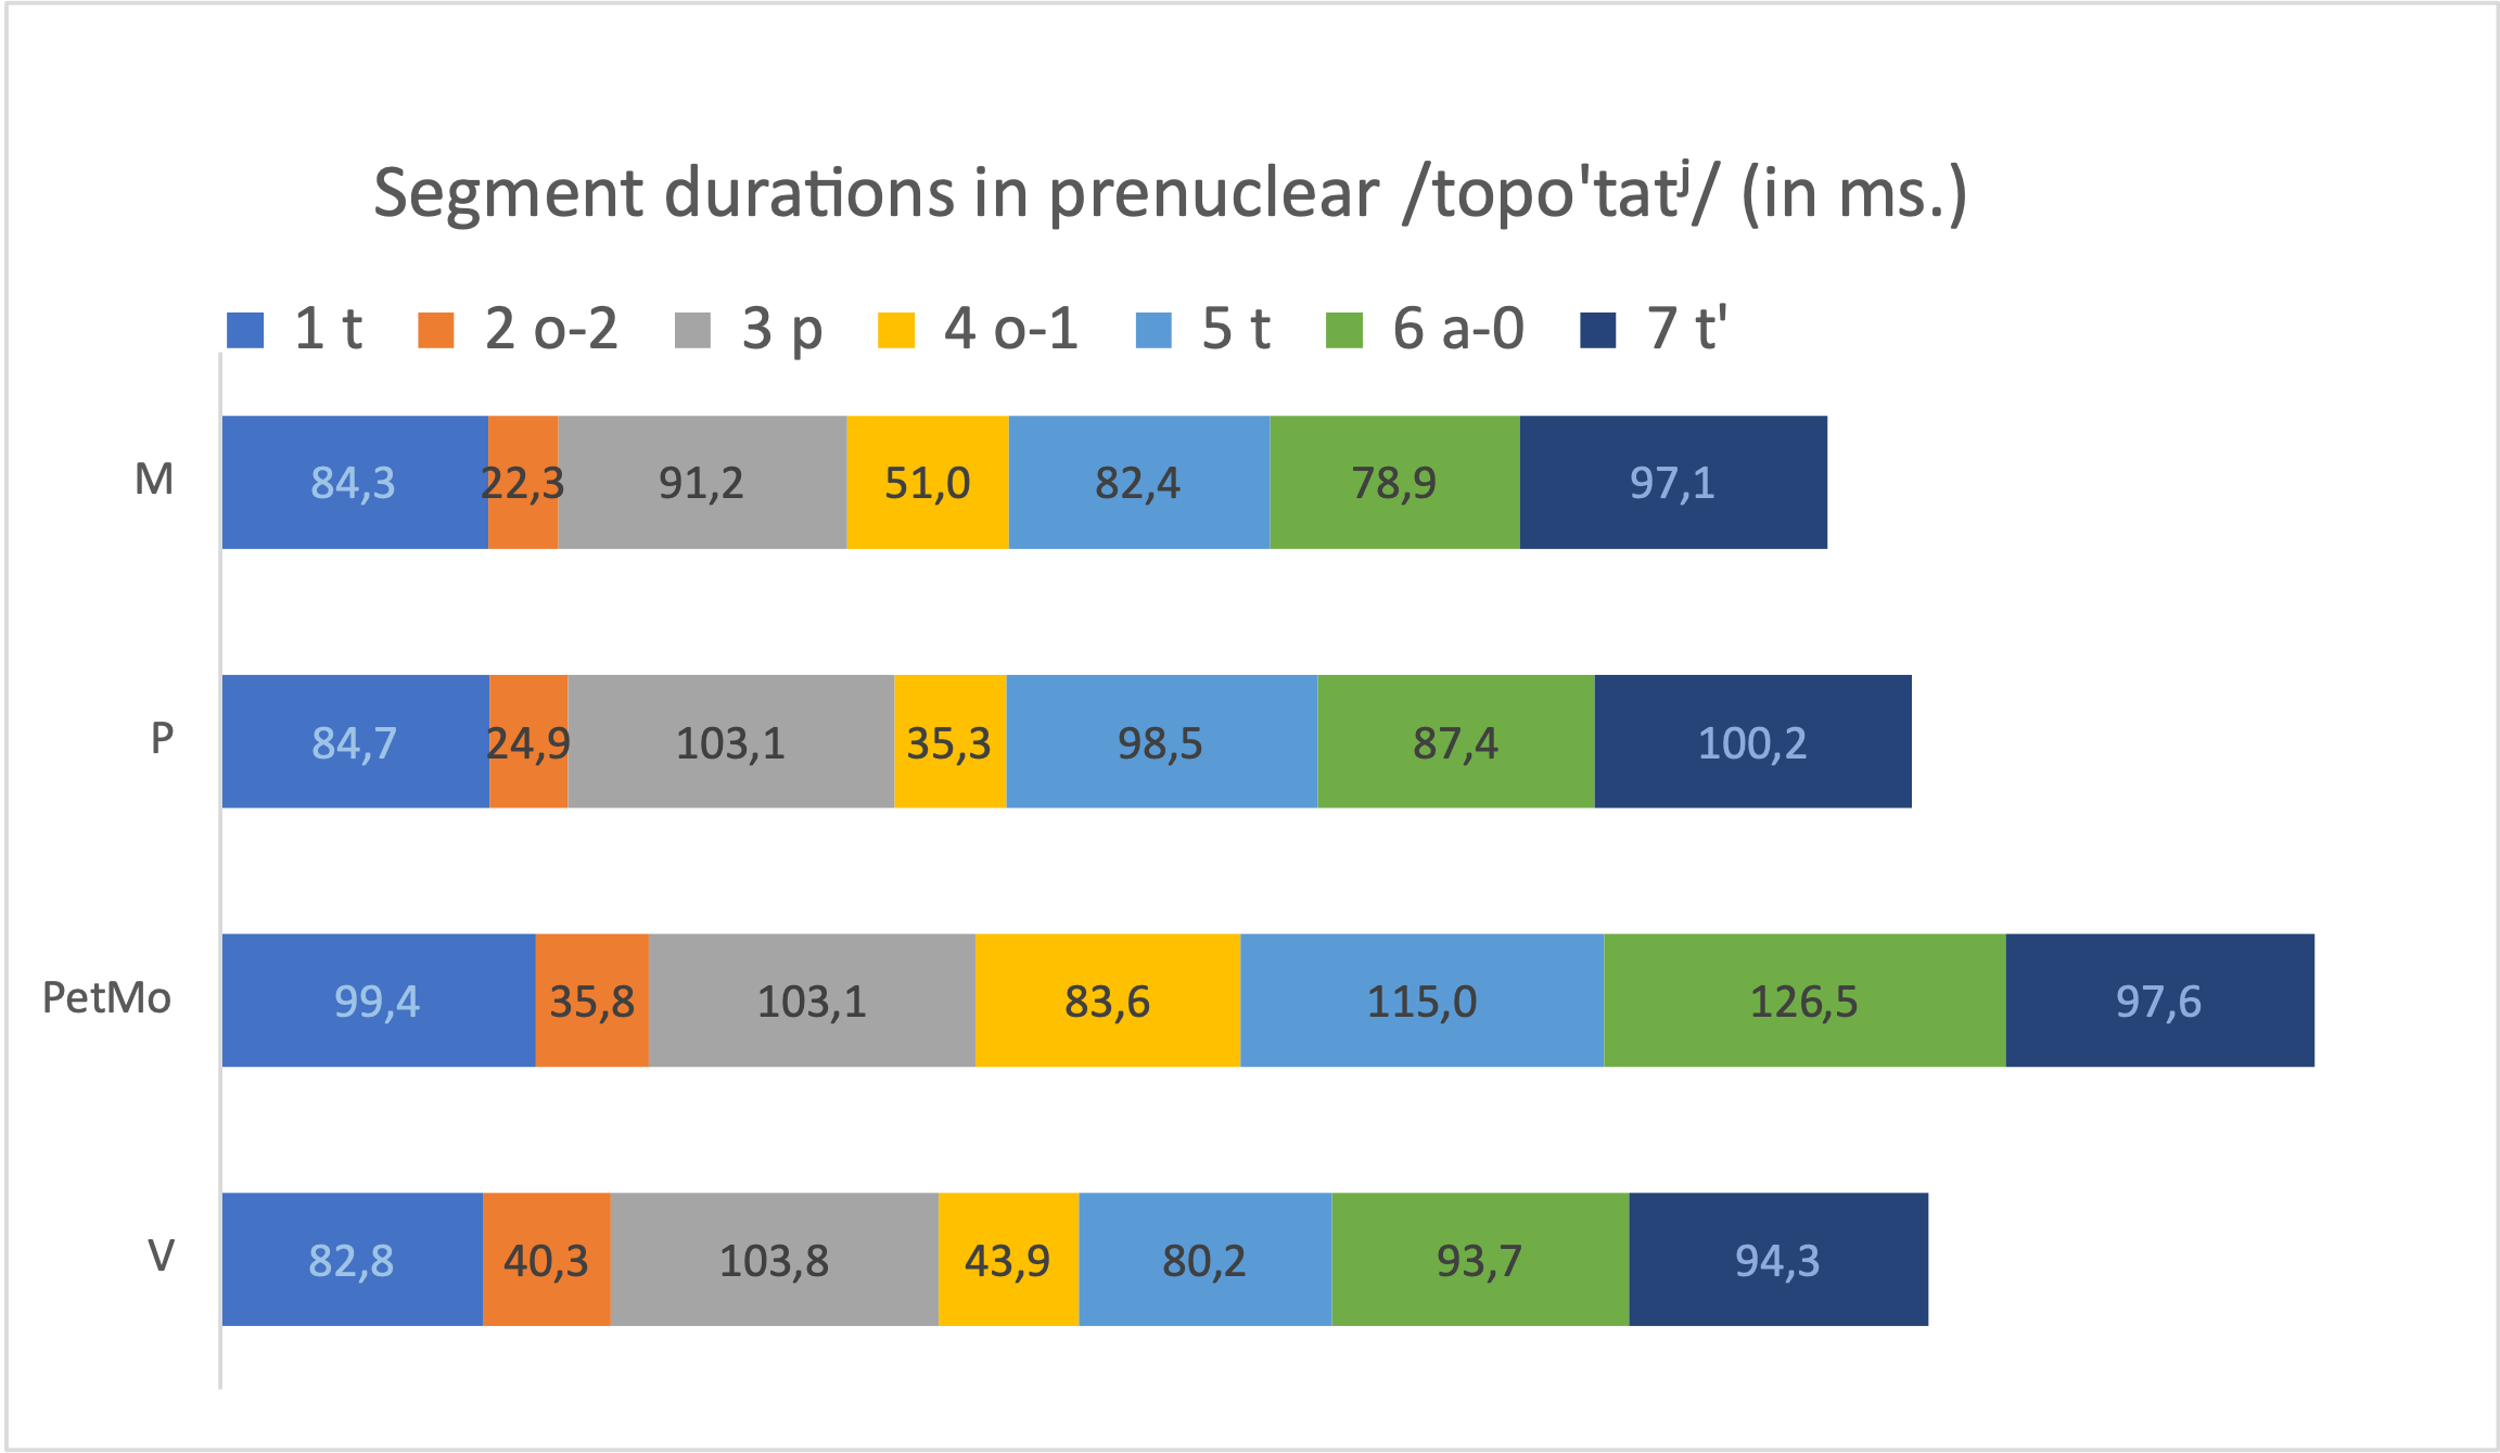
\includegraphics[width=\textwidth]{post-img007a.png}
\begin{subfigure}{\textwidth}
    \pgfplotstableread{data/post-figure7a.csv}\PostFigureSevenAData
    \pgfplotsset{cycle list/RdYlBu-7}
    \begin{tikzpicture}
	\small
	\begin{axis}
		[
            axis lines*=left,
			font=\small,
			height=7cm,
			nodes near coords,
			point meta=x,
			visualization depends on={rawx \as \rawx},
			every node near coord/.style={
				black,
				font=\footnotesize\bfseries,
				xshift=-\rawx*.25,
				yshift=3ex
			},
			legend cell align=left,
			legend columns=-1,
			legend to name=CustomLegendPosA,
			width=\textwidth,
			ytick=data,
			y dir=reverse,
			xtick=\empty,
			yticklabels from table={\PostFigureSevenAData}{Data},
            xbar stacked,
			xlabel=ms,
			ylabel near ticks,
			xmin=0,
			bar width=4ex,
			enlarge y limits=0.25,
			every axis plot/.append style={fill},
			cycle list name=RdYlBu-7
		]
		\foreach \i in {1 t,2 o-2,3 p,4 o-1,5 t,6 a-0,7 t'}
		  {
		  	\addplot table [y expr=\coordindex, y=Data, x=\i, point meta=\thisrow{\i}] {\PostFigureSevenAData};
		    \edef\temp{\noexpand\addlegendentry{\i}}
		    \temp
 		  }
	\end{axis}
	\node[anchor=base] at (current axis.above north) {\ref{CustomLegendPosA}};
    \end{tikzpicture}
\caption{Segment durations in prenuclear /topoˈtatʲ/ (ms)}
\end{subfigure}\medskip\\
\begin{subfigure}{\textwidth}
    \pgfplotstableread{data/post-figure7b.csv}\PostFigureSevenBData
    \pgfplotsset{cycle list/RdYlBu-7}
    \begin{tikzpicture}
	\small
	\begin{axis}
		[
            axis lines*=left,
			font=\small,
			height=7cm,
			width=\textwidth,
			ytick=data,
			xtick=\empty,
			yticklabels from table={\PostFigureSevenBData}{Data},
            xbar stacked,
			xlabel=\%,
			ylabel near ticks,
			y dir=reverse,
			xmin=0,
			xmax=100,
			bar width=4ex,
			enlarge y limits=0.25,
			every axis plot/.append style={fill},
			cycle list name=RdYlBu-7
		]
		\foreach \i in {1 t,2 o-2,3 p,4 o-1,5 t,6 a-0,7 t'}
		  {
		  	\addplot table [y expr=\coordindex, y=Data, x=\i] {\PostFigureSevenBData};
 		  }
	\end{axis}
% % % 	\node[anchor=base] at (current axis.above north) {\ref{CustomLegendPosB}};
% We don't need a legend here as the one from A is also valid for B.
    \end{tikzpicture}
\caption{Segment durations in prenuclear /topoˈtatʲ/ (in \% of total word)}
\end{subfigure}

% % % 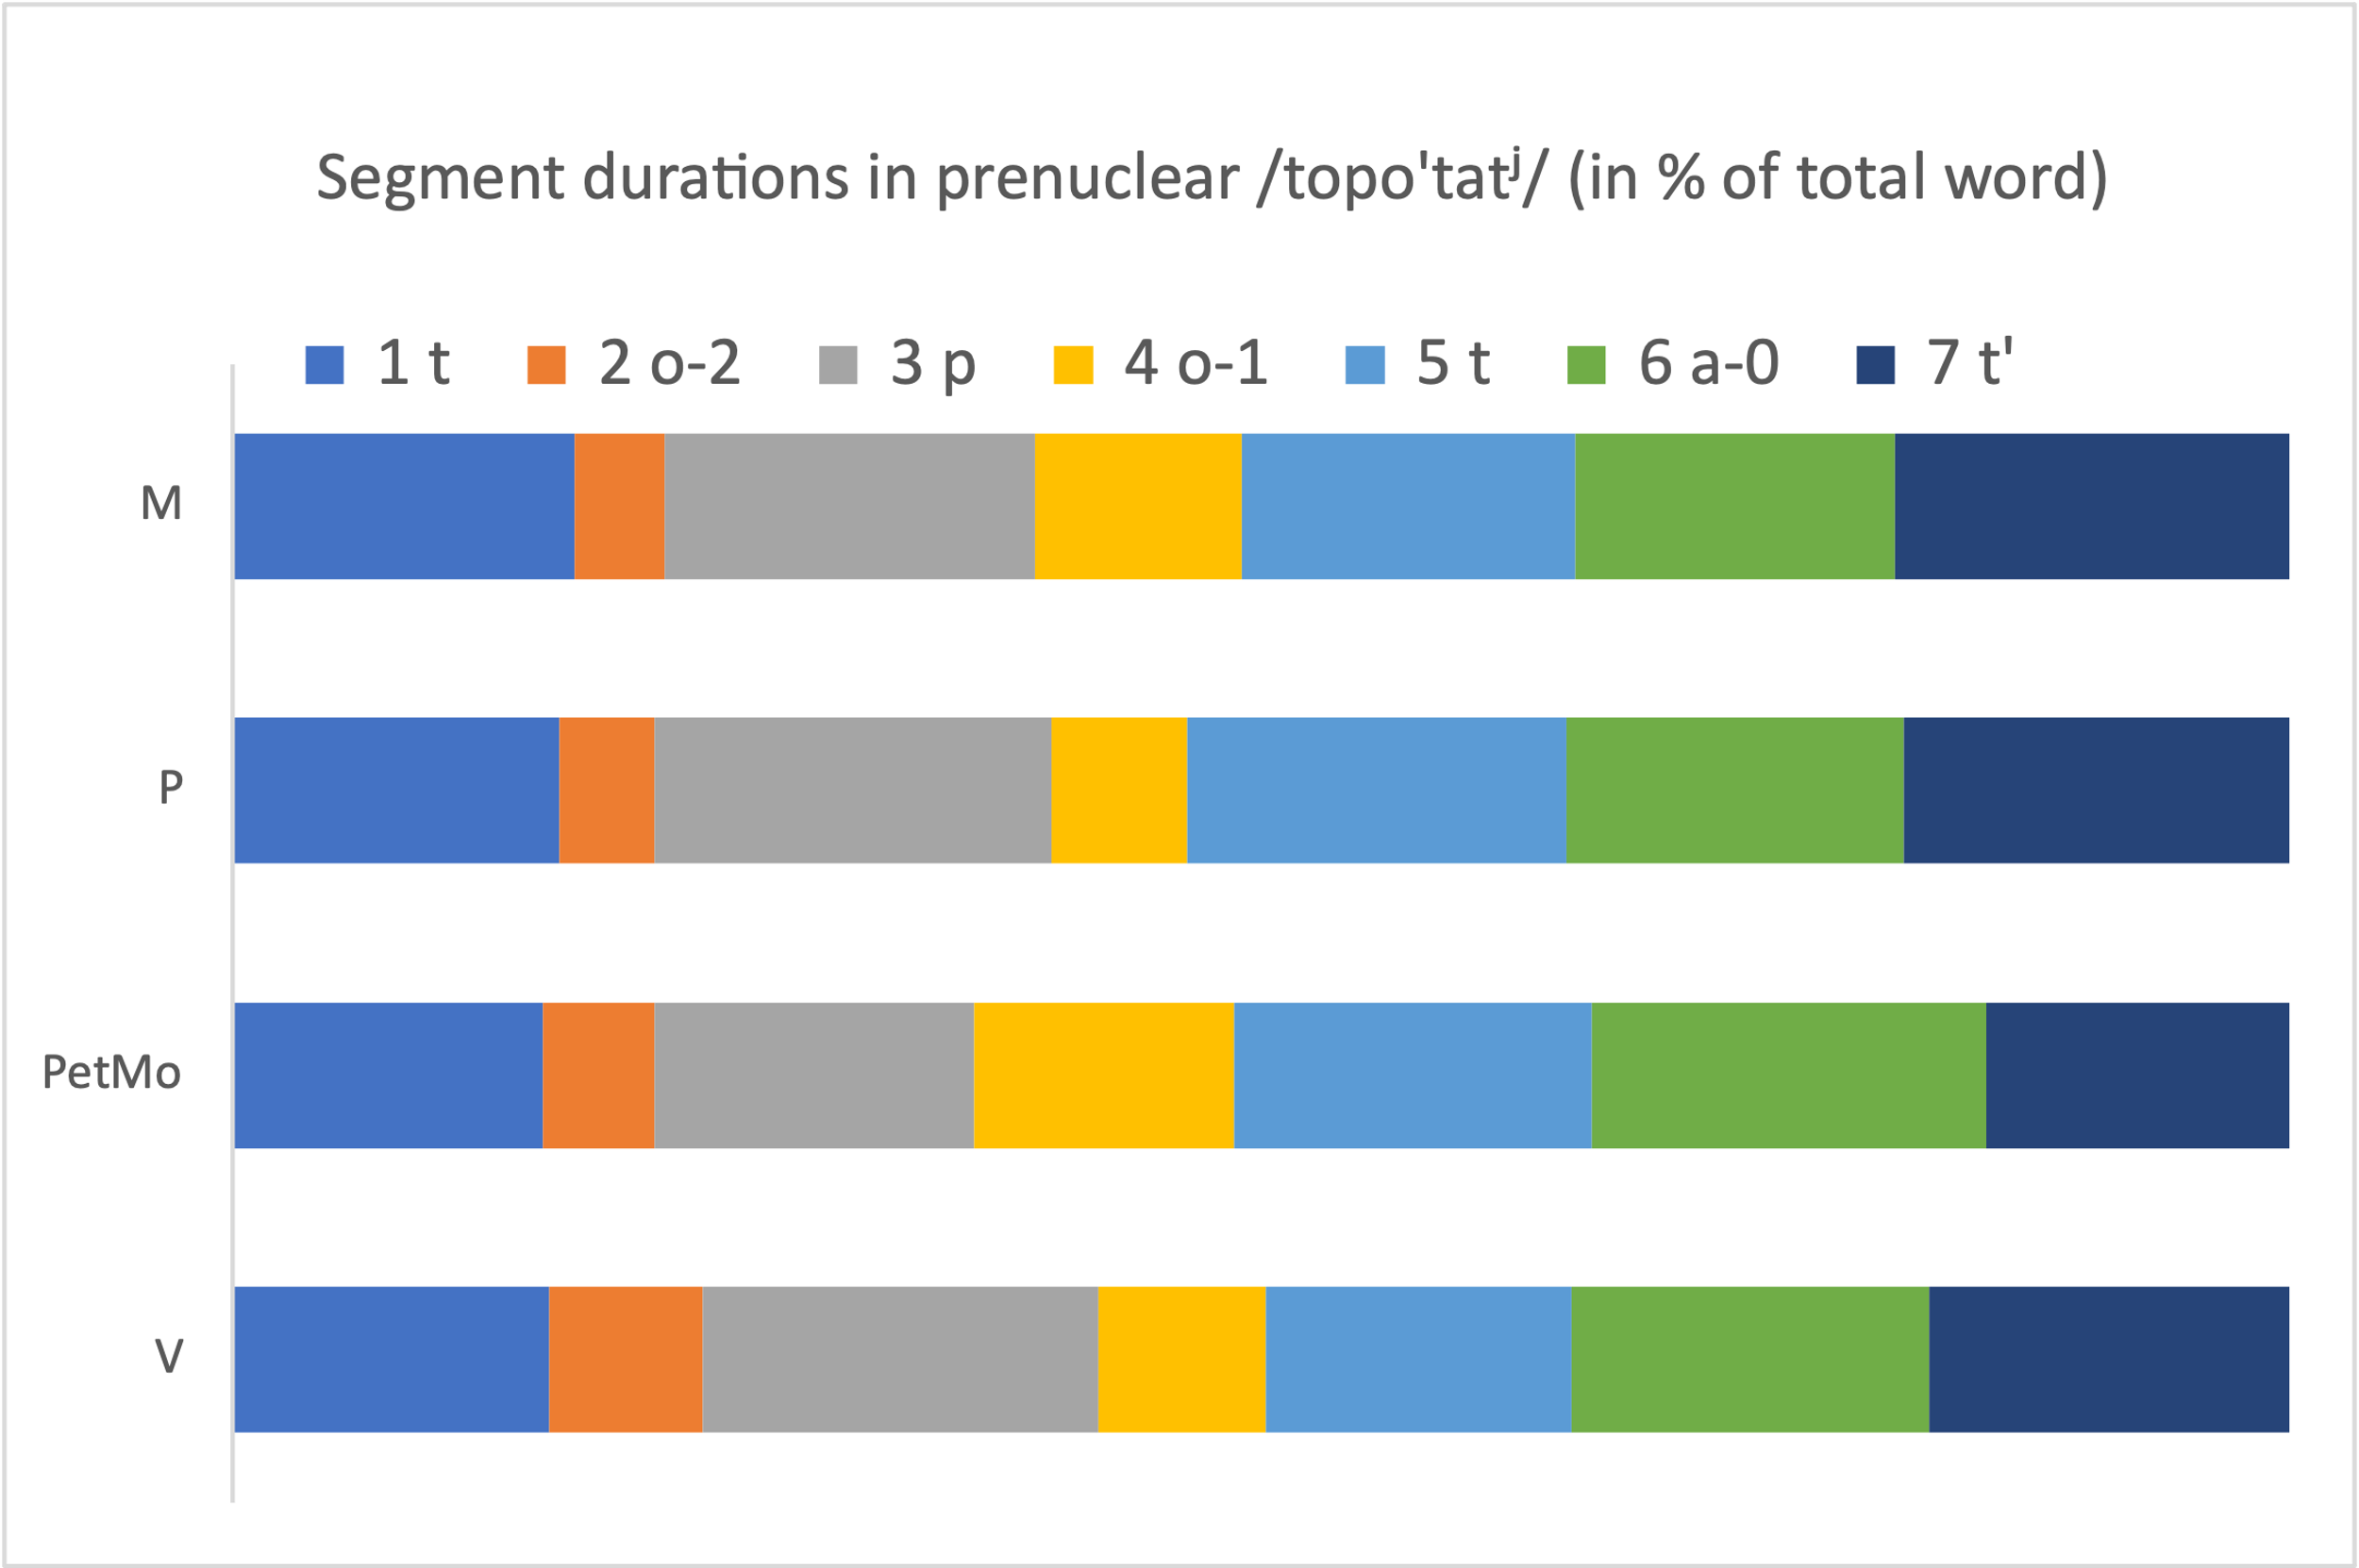
\includegraphics[width=\textwidth]{post-img007b.png}
\caption{\label{fig:post:7} Durations of all consonants and vowels in \textit{topotát'} in utterance \REF{ex:post:2}, in milliseconds (upper graph) and relative to the duration of the whole word (lower graph). The upper row M shows the mean values for all 13 speakers from Moscow, the second row P for the 13 speakers from Perm. Row 3 (PetMo) gives the values for a teacher of Russian, and row 4 (V) for an adolescent from the Vologda region (Northern Russia). The numbers in the upper graph give the mean durations in milliseconds.}
\end{figure}


The numbers on which this figure is based are limited (one word production per speaker, so $n = 13$ for row 1 (Moscow) and $n = 13$ for row 2 for Perm), but there can be no doubt about the general picture that consonants are longer than vowels in unstressed syllables in both cities. The teacher I recorded (PetMo, third row), who is more than 40 years older than the other participants, has much longer vowels, both in milliseconds and relative to the other segments in the word (and not only in this utterance), but even in her speech, the unstressed consonants are longer than the vowels. In \citegen{Vysotskij1973} data, a\textsubscript{$-1$} has the same duration as the preceding consonant in CSR, but it is much longer in groups II and V.\footnote{\citet{Vysotskij1973} measured not only vowel durations in 15 different dialect groups, but also the durations of the surrounding consonants (1973: 39--40, Figs. 2 and 3), but he did not discuss the consonantal durations.} The patterns in groups VIII and IX are again more like the Perm pattern.



Our Muscovite speakers obviously did not use the extremely prominent first pretonic vowels which the old Moscow dialect and Moscow vernacular speech are known for (\citealt{Vysotskij1973, Lapteva1999}), but they are still long compared to the second pretonic vowels.


\subsection{Two-degree reduction in East-Slavic: Strong centre and weak periphery}
\label{sec:post:4.3}
The durational reduction in two degrees is claimed to be a feature shared by all three East Slavic languages \citep{Dubina2012}, but the difference between second and first pretonic vowels is small among speakers of Ukrainian from the west of Ukraine, at a long distance from Central Russia \citep{ŁukaszewiczEtAl2022}.\footnote{The word prosodic pattern in Ukrainian is complicated by iterative secondary stresses (\citealt{ŁukaszewiczMołczanow2018}).} Earlier literature on rural dialects in Russia (cf. \sectref{sec:post:1.2.2}) suggested that the relative difference between the two pretonic vowels is strongest in a central region of the East Slavic dialect continuum, and gets weaker when moving from the centre, and that this difference is retained in modern urban Russian (cf. \sectref{sec:post:1.2.3}). Our data, although representing only two cities, is in line with these earlier, preliminary observations.


\subsection{Sociolinguistic dimension}
\label{sec:post:4.4}
\subsubsection{Gender}
\label{sec:post:4.4.1}
Our remaining research questions concern possible gender effects, first on overall vowel duration: Do the girls have longer vowel durations than the boys, as female speakers tend to have in many other languages? This is true for the female speakers in Perm, but not for the female speakers in Moscow, who use almost the same vowel durations as their male classmates, for all vowels in general, and also for each individual position (cf. \sectref{sec:post:3}).



The scarce literature on gender effects on phonetics in Russian suggests that the girls might have longer pretonic vowels than the boys, and that the Perm girls might have a vowel reduction pattern that is more similar to the Moscow speakers and to the Central Standard Russian norm than the Perm boys, in case it is true that they speak closer to a non-local norm (see \sectref{sec:post:1.2.4} above). Neither can be found in our data. The girls do not use stronger first pretonic lengthening than the boys, nor do the girls in either city show less local colouring than their male peers, as young urban women often do in other countries \citep{Labov2001}, at least not in their word prosodic structure, which might be less conscious than other, more salient features, such as the stigmatised pronunciation of [o] in unstressed position \citep{Andrews1995}, which is avoided in formal speech \citep{Erofeeva1993}. In their question intonation, however, the same girls in Perm did indeed speak with less colouring than the boys, as we found in a recent study of the same speakers \citep{RN1173}.



These results should preferably be confirmed with larger data sets from more speakers. We have no guarantee that our 13 speakers from a single school in Moscow and their peers in Perm are representative for todays' youth from the two cities.


\subsubsection{Other sociolinguistic variables}
\label{sec:post:4.4.2}
As to other sociolinguistic parameters, we did not study the role of education, since almost all adolescents had parents with a high education level and they were still at school age themselves. We did not focus on age either, but one of our participants – the teacher from Saint Petersburg and Moscow – was more than 40 years older than the pupils from Moscow and Perm. It is no surprise that her vowels were much longer, since young people tend to have a faster articulation rate. More interesting for our research question is that the teacher also had a much larger difference between the pretonic vowels, due to her relatively long first pretonic vowels. Her two-degree reduction is closer to the vernacular Moscow speech and the older Moscow norm that Vysotskij recorded more than fifty years ago (\figref{fig:post:1}, groups II and III). It is stronger not only than in today’s adolescent speech, but even stronger than in \citegen{Vysotskij1973} pattern for Central Standard Russian (\figref{fig:post:1}, group I), so she has relatively strong local colouring in her word rhythm pattern.


\subsubsection{Even in read speech}
\label{sec:post:4.4.3}
The results show a remarkable difference between the cities, even though the data are obtained from read speech. Speaking style has a major effect on the frequency of unreduced, [o]-like pronunciations of unstressed \mbox{/o/} among speakers from Perm, ranging from 4\% in read speech to 69\% in spontaneous speech (\citealt{VerbickajaEtAl1984, Erofeeva1993}, cf. \sectref{sec:post:1.2.4}). 



Both \citet{Vysotskij1973} and \citet{Erofeeva2005} used data from spontaneous speech, which tends to show a higher degree of local colouring than read speech, and Erofeeva’s speakers were even known to have a local accent, for which our speakers have not been screened. Therefore, it is remarkable that our data show the same high degree of local colouring as Erofeeva’s spontaneous data, even though our recordings are from formal, read speech. This supports the suggestion that reduction in only one degree is not considered a serious violation of standard Russian, only of orthoepic rules (\citealt{Bondarko1998}, cf. \sectref{sec:post:1.2.4} above), unlike the production of unstressed \mbox{/o/} as [o], and thus of lack of reduction, which is actively avoided in read speech. It is highly probable that the rhythmic feature we studied is less stigmatised than more salient dialect traits (cf. \citealt{GrammatčikovaPožarickaja2013}: 72). 


\section{Conclusions}
\label{sec:post:5}
Our study of relative vowel durations in prestressed position among young urban Russians from Moscow and from Perm shows that we do find regional variation in modern-day Russian urban speech, at least in prosody: All Moscow speakers make a clear distinction between two degrees of reduction, whereas the speakers in Perm hardly differentiate the second and first pretonic vowels. In speech by speakers from Perm we see very little first pretonic vowel prominence. In this regard, the Perm variety is in fact close to the most extreme rural dialects, which do not have, or hardly have, reduction in two degrees. This regional distinction between Moscow and Perm speech is very stable. There is no effect of gender, and it is maintained even in read speech, where the tendency to suppress regional dialect traits is strongest. Apparently, whereas the production of unreduced [o] is actively avoided, and/or on its way out of Perm speech, vowel reduction in only one degree is not.



The two-degree reduction in quantity appears to be categorical for our Moscow speakers. Our data do not suggest that this is the case in Perm. Although we do find a small difference in quantity in Perm, this difference is not statistically significant, and the degree of variation is very high. The small difference we see in average values need not be a categorical distinction, only a gradual tendency to be somewhat longer.



It would be no surprise if today’s Moscow youth speak with less local accent than previous generations. Still, although the first pretonic is never that prominent as in the extreme cases Moscow speech is known for, they retain a very distinct two-degree reduction. The relative difference between first and second pretonic is large, and larger than in many previous recordings of Central Standard Russian speech, due to the extremely short second pretonics among our Moscow speakers. It will be interesting to observe the further development and the social status of a Moscow accent, both in and outside Russia, in the current, changing world.



Although only covering two cities, our data are in line with previous observations of an opposition between centre and periphery in the East Slavic dialect continuum in the expression of the word prosodic structure. A difference between strong pretonic prominence in the central area and weaker prominence in non-central areas is still found in modern urban Russian.



In future research, data from more cities should be added. Moscow and Perm might be extremes on a scale, since both cities are known for a relatively strong local accent. When \citet{GrammatčikovaPožarickaja2013} claimed that Russians often can distinguish speakers from different cities, they mentioned three cities as examples: Bryansk (Western Russia, not far from Belarus and Ukraine), Perm (Ural region) and Moscow. I suspect that these cities are not chosen randomly, but because they are known for their local features.


\section*{Acknowledgements}

The author is obliged to the following people for support in various stages of the research: First of all, to Benedikte Fjellanger Vardøy for doing the recordings in Perm and for fruitful cooperation in an earlier analysis of the vowels, further to Svetlana Djačenko for doing most of the segmentations and to Bistra Andreeva for statistical analyses and advice. I would also like to thank Alexander Krasovitsky, Sergej Knjazev, Elena Erofeeva, Brechtje Post, Elaine Schmidt and Dirk Jan Vet for advice on phonetics at different stages of this research, the members of the Phonetics group at Saarland University for their hospitality and advice during my research stay in 2022, and the two anonymous reviewers for valuable response. I remain responsible for all remaining shortcomings. Last but not least, I thank the speakers and the secondary schools in Moscow and Perm they attended for their participation. 



This research was supported by various grants from the University of Bergen and by the Meltzer Foundation in Bergen, Norway. The data collection has been approved by the Norwegian Social Science Data Services (NSD).


\sloppy\printbibliography[heading=subbibliography,notkeyword=this]
\end{document}
